%!TEX root = ../main.tex

\graphicspath{{./figures/chapter5/}}

\chapter{RNA localization by the numbers}
\label{ch:chapter5}

\minitoc
\newpage

In this chapter we present several applications of the pipeline described in the previous chapters.
More specifically, we analyze experimental datasets in order to explore, quantify and validate biological insights about \ac{mRNA} localization.
Results from this chapter are computed from three different high content screening studies, totaling tens of transcripts observed through thousands of bioimages.

In the first section, we develop a general classification pipeline to identify generic \ac{mRNA} localization patterns from \ac{smFISH} images~\cite{CHOUAIB_2020}.
In the second section, exploiting the same dataset, we focus on a specific and novel clustering pattern: the translation factories.
These first two sections describe the work published in:

\begin{center}
	\color{green}
	R. Chouaib, A. Safieddine, et al. (2020), \textit{A dual protein-mRNA localization screen reveals compartmentalized translation and widespread co-translational RNA targeting}, Developmental Cell 54 (6), 773.
\end{center}

In the third section, we exploit a \ac{GFP} channel to visualize and detect centrosomes.
We observed a centrosomal localization patterns for different transcripts and different mitosis phases~\cite{safieddine_choreography_2021}.
This work was published in:

\begin{center}
	\color{green}
	A. Safieddine, E. Coleno, et al. (2021), \textit{A choreography of centrosomal mRNAs reveals a conserved localization mechanism involving active polysome transport}, Nature Communications 12 (1), 1352.
\end{center}

In the fourth section, we detail several transcripts with a protrusion localization pattern~\cite{pichon_kinesin_2021}.
This last section mainly describes results presented in:

\begin{center}
	\color{green}
	X. Pichon, K. Moissoglu, et al. (2021), \textit{The kinesin KIF1C transports APC-dependent mRNAs to cell protrusions}, RNA 27 (12), 1528.
\end{center}

\section{A systemic quantification of RNA localization}
\label{sec:general_pattern_recognition}

In~\cite{CHOUAIB_2020} I have implemented a quantitative pipeline to analyze the localizations of \ac{mRNA} molecules.
This work lays the foundation of the future Python packages developed in FISH-quant V2~\cite{Imbert_fq_2022}.
My contribution consists in classifying individual cells with one or several \ac{RNA} localization patterns.

\subsection{Introduction}
\label{subsec:introduction_general_pattern}

Most of \ac{mRNA}s have a random distribution throughout the cytoplasm, but some of them localize in specific subcellular regions.
This phenomenon has been previously reviewed in different papers~\cite{Blower_2013, Jung_2014, Eliscovich_2017, Bovaird_2018}.

Such localization can be related to either the \ac{RNA} metabolism, for example with untranslated \ac{mRNA}s stored and repressed in \ac{P-bodies} (but not degraded~\cite{Hubstenberger_2017}), or the protein metabolism with locally translated proteins.
This local synthesis concerns both mature proteins and nascent peptides.
Different cellular processes imply the delivery of mature proteins in specific subcellular regions and a local regulation of the proteome.
Local translation can contributes to cell fate determination during metazoan development, as observed in~\cite{melton_translocation_1987} with a clear modification of the Vg1 \ac{RNA} spatial distribution between mature and immature Xenopus oocytes.
In these same Xenopus embryos, cyclin B1 \ac{mRNA}s localized at the mitotic apparatus could also play an important role in the rapid cell division cycles observed during early embryogenesis~\cite{Groisman_2000}.
In mammal cells, \ac{RNA} localization influences cell polarization and motility, usually through actin localization at the cell edge~\cite{Lawrence_1986}.
Locally translated proteins are also known to be involved in axonal growth and so neural plasticity~\cite{VanDriesche_2018}.
Finally, by precisely controlling the \ac{mRNA} localization and the subsequent translation process, cells can avoid to release proteins at inappropriate places~\cite{Muller_myelin_2013} and help the synthesis of protein complexes~\cite{pichon_visualization_2016}.

Several mechanisms will drive the localization of \ac{mRNA}s.
Sometimes the nascent peptide can serve as a targeting signal, but most of the time the \ac{RNA} molecule itself will initiate its localization.
\ac{RNA} can also be trapped in specific subcellular compartments.
The molecule often include a zip-code sequence that is read by a \ac{RBP} and starts the assembly of a transport complex comprising different organelles or motor proteins.
Such complex can then directly convey the \ac{RNA} along the cytoskeleton~\cite{Blower_2013}.
Coupled with an anchoring mechanism at the targeted destination, it provides a better stability of the \ac{RNA} localization.

In~\cite{CHOUAIB_2020}, we claim that a global view of local translation in the whole cell and at the genomic level is still to come, despite recent progress.
In a pioneering work on Drosophila embryogenesis~\cite{lecuyer_global_2007}, authors analyze 3,370 genes and find that 71\% of them encode a transcript with a non-uniform localization pattern.
In human cell lines recent studies exploit and improve \ac{smFISH} techniques to image thousands of \ac{mRNA}s in the perinuclear region, the mitochondria and the cell membrane~\cite{battich_image-based_2013, Chen_2015, eng_seqfish_2019, Xia_2019}.
We take a step forward in studying \ac{mRNA} localization with human cell lines and a systematic approach.
We perform a quantitative analysis leveraging supervised and unsupervised methods in order to recognize up to 6 different localization patterns.
The current section emphasizes this quantitative pipeline that contributes to make our analysis scalable and more robust.

\subsection{Materials and methods}
\label{subsec:materials_general_pattern}

The quantitative pipeline used in this study and the existing work in FISH-quant V1 are the building blocks of FISH-quant V2.
Therefore, the various methods presented here were not yet packaged in \emph{bigfish}, but Python libraries that formed its foundation are already in used.
This work is developed in Python and the code repository is public\footnote{\url{https://github.com/Henley13/paper_translation_factories_2020}}.

\subsubsection{Experimental data}

At first more than 500 genes have been manually analyzed to identify potential transcripts with non random localization patterns within the cell.
In addition to different qualitative and manual observations performed over this dual \ac{RNA}-protein localization screen, we also develop a quantitative pipeline to systematically classify transcripts' localization patterns.
To this end, I exploit a dataset of 526 \ac{FoV}s, combining DAPI and \ac{smFISH} channels as illustrated in Figure~\ref{fig:fov_racha}.
The raw images stacks several 2D acquisitions to gather a 3D information of the \ac{FoV} with a z-spacing of 0.3μm.
Acquisitions are performed with a Zeiss Axioimager Z1 widefield microscope or a Nikon Ti fluorescence microscope, on human cell lines HeLa.
In total, this dataset is built from 57 independent experiments gathering observations from 27 different \ac{mRNA}s under different experimental conditions.

\begin{figure}[]
    \centering
    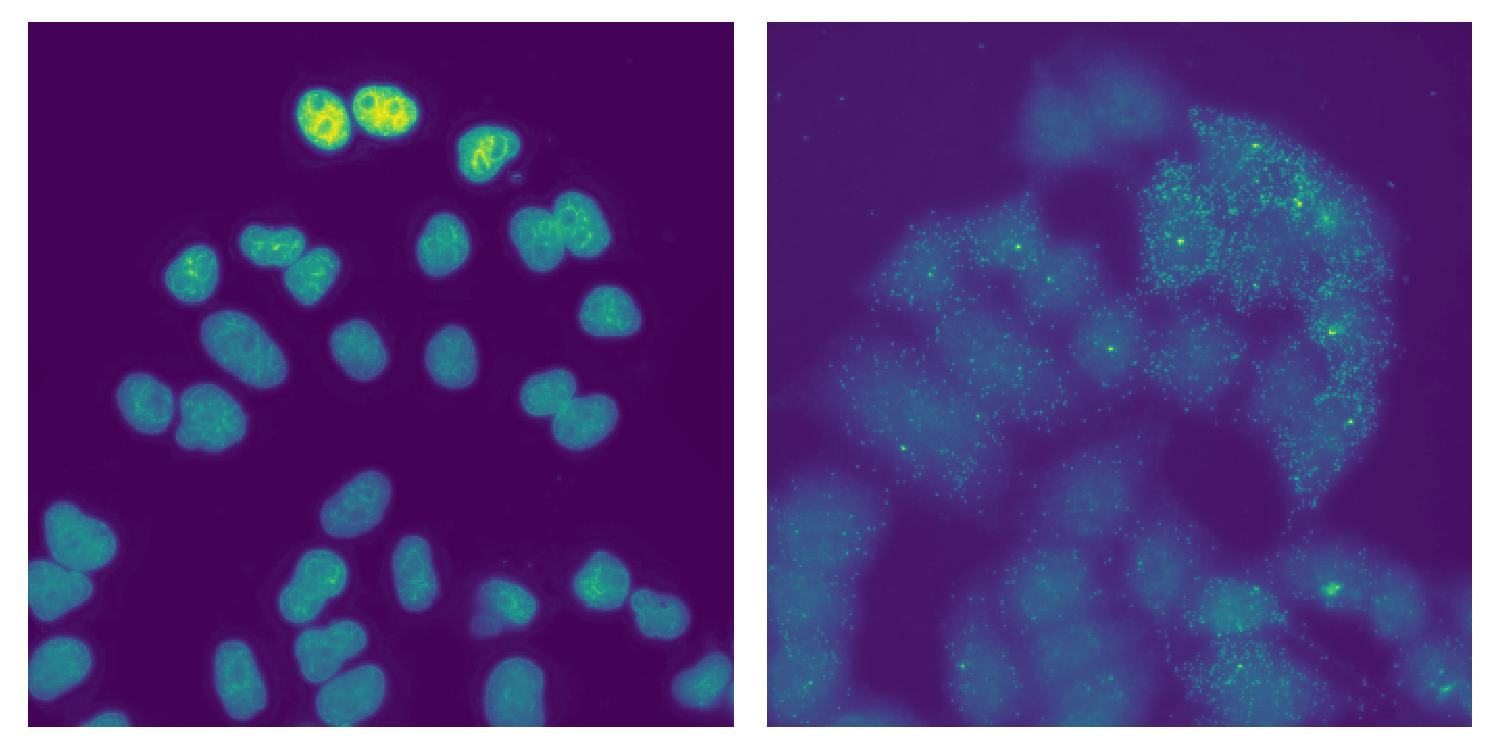
\includegraphics[width=\textwidth]{figures/chapter5/FoV_DYNLL2}
    \caption{Contrasted image with Dapi (\textit{left}) and smFISH (\textit{right}) channels.
	Images are projected in 2D.
	Targeted transcript is DYNLL2.
	Plot build with \emph{bigfish}}
    \label{fig:fov_racha}
\end{figure}

\subsubsection{Semi-automated RNA detection}

\ac{RNA} detection is performed with a Python implementation of FISH-quant v1~\cite{mueller_fish-quant_2013}.
I apply a \ac{LoG} filter on the 3D \ac{smFISH} images, then a local maximum detection algorithm.
However, a threshold value has to be set manually for every experiment to discriminate the actual spots from the noisy background blobs.
Large agglomeration of spots are decomposed with a gaussian mixture model, following~\cite{samacoits_computational_2018}.
Ultimately, \ac{RNA} clusters - namely foci - are detected with a DBSCAN algorithm~\cite{ester_density-based_1996} applied on the detected spots.
According to the way a DBSCAN cluster samples, a foci is then defined as a set of at least 5 points where for each point there is at least one other point from the foci within a 350 nanometers distance.
All foci overlapping the nuclear area in the projected 2D images are considered as a transcription site and removed from the analysis.
Percentages of \ac{RNA} in foci are then calculated as number of \ac{RNA} inside the cytoplasmic foci divided by the number of cytoplasmic \ac{RNA}s.

There are two main differences compared to the current detection methods implemented in FISH-quant and presented in Chapter~\ref{ch:chapter2}: a detection threshold has to be set manually and the decomposition of agglomerated spots has since been simplified.

\subsubsection{Cell and nucleus segmentation}

Nucleus segmentation is performed from the DAPI channel and cell segmentation from the cell autofluorescence in the \ac{smFISH} channel.
Segmentation is performed in 2D for both nuclei and cells, thus 3D images are projected in two dimensions using their maximal local focus values~\cite{tsanov_smifish_2016}.

Nuclei are segmented with NucleAIzer~\cite{hollandi_nucleaizer_2020}, a deep neural network pipeline trained with the annotations from the Data Science Bowl 2018 challenge\footnote{\url{https://www.kaggle.com/c/data-science-bowl-2018}}.
This pipeline is based on a Mask R-CNN architecture~\cite{He_2017_ICCV}, with optionally a fine-tuning of the segmented boundaries with a U-Net model~\cite{Ronneberger_unet}.
After a first round of segmentation, some nuclei are missing, so I remove the segmented nuclei from the DAPI channel and feed NucleAIzer with the remaining nuclei for a second round of segmentation.
Removing the segmented nuclei from the original image implies some morphological mathematics techniques as described in Chapter~\ref{ch:chapter3}.
This technique is now implemented in FISH-quant.

Cells are segmented with a watershed algorithm using nuclei masks as seeds.
A threshold value is set manually for every experiment to discriminate the cell surface from the background.
In case of poor results, some segmentation masks are corrected manually.
This is especially the case for transcript that tend to localize in cell protrusion.
Indeed, such localization pattern is highly sensitive to the segmentation accuracy.

\subsubsection{Localization feature engineering}

Based on the segmentation masks and the coordinates of the detected spots, I identify 9,710 individual cells with an average of 346 \ac{RNA}s per cell.
For each cell, I collect the cell and nucleus masks in 2D, the \ac{RNA} and the potential clusters coordinates in 3D.
In addition I save an image of the cell, for visualization purpose, and different information about the experiment (the presence of a treatment, the targeted gene, etc.).
Cropped cells, empty cells or cells with less than 30 \ac{RNA} detected inside are removed.
At this point, I have a coordinate representation of every cell, as presented in Chapter~\ref{ch:chapter4}.

I design and compute a set of 15 features to describe the spatial distribution of points inside the cell:
\begin{itemize}
	\setlength\itemsep{0.1em}
	\item The number of foci.
	\item The proportion of \ac{RNA} inside foci.
	\item The proportion of \ac{RNA} inside the nucleus.
	\item The average \ac{RNA} distance to the cell membrane, normalized by the value obtained under a uniform \ac{RNA} distribution.
	\item The average \ac{RNA} distance to the nucleus membrane, normalized by the value obtained under a uniform \ac{RNA} distribution.
	\item The average foci distance to the cell membrane, normalized by the value obtained under a uniform foci distribution.
	\item The average foci distance to the nucleus membrane, normalized by the value obtained under a uniform foci distribution.
	\item The proportion of \ac{RNA} inside cell protrusion.
	A protrusion region is defined by calculating the difference between the segmented cellular region and its morphological opening with a large window.
	\item The peripheral dispersion index, defined as the squared point distance to the centroid of the cell and normalized by the value obtained under a uniform \ac{RNA} distribution.
	\item The number of \ac{RNA}s within 515 nm from the nucleus membrane, normalized by the value obtained under a uniform \ac{RNA} distribution.
	\item The number of \ac{RNA}s between 515 nm and 1030 nm from the nucleus membrane, normalized by the value obtained under a uniform \ac{RNA} distribution.
	\item The number of \ac{RNA}s between 1030 nm and 1545 nm from the nucleus membrane, normalized by the value obtained under a uniform \ac{RNA} distribution.
	\item The number of \ac{RNA}s between 0 nm and 515 nm from the cell membrane, normalized by the value obtained under a uniform \ac{RNA} distribution.
	\item The number of \ac{RNA}s between 515 nm and 1030 nm from the cell membrane, normalized by the value obtained under a uniform \ac{RNA} distribution.
	\item The number of \ac{RNA}s between 1030 nm and 1545 nm from the cell membrane, normalized by the value obtained under a uniform \ac{RNA} distribution.
\end{itemize}

The apparent precision of the nanometer distances is just an artifact as the concentric regions are delimited visually from a sample of cell images.
Therefore, the width of these regions are defined in pixels, more precisely, with a 5 pixels width and a pixel size of 103 nm.

\subsubsection{Binary classification models}

\begin{figure}[]
	\centering
	\minipage{0.2\textwidth}
		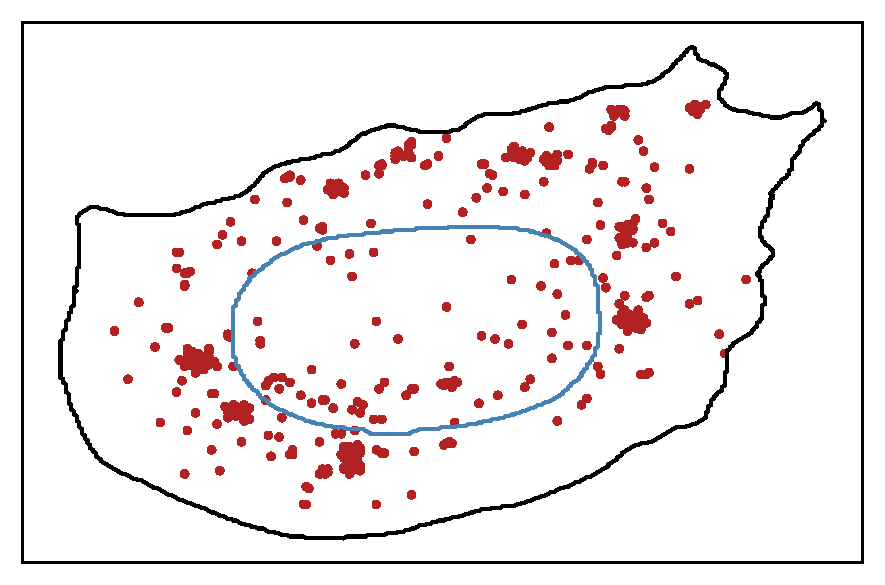
\includegraphics[trim={0.5cm 0.5cm 0.5cm 0.5cm},clip,width=\linewidth]{figures/chapter5/plot_foci}
		\subcaption{Foci}
	\endminipage\hfill
	\minipage{0.2\textwidth}
		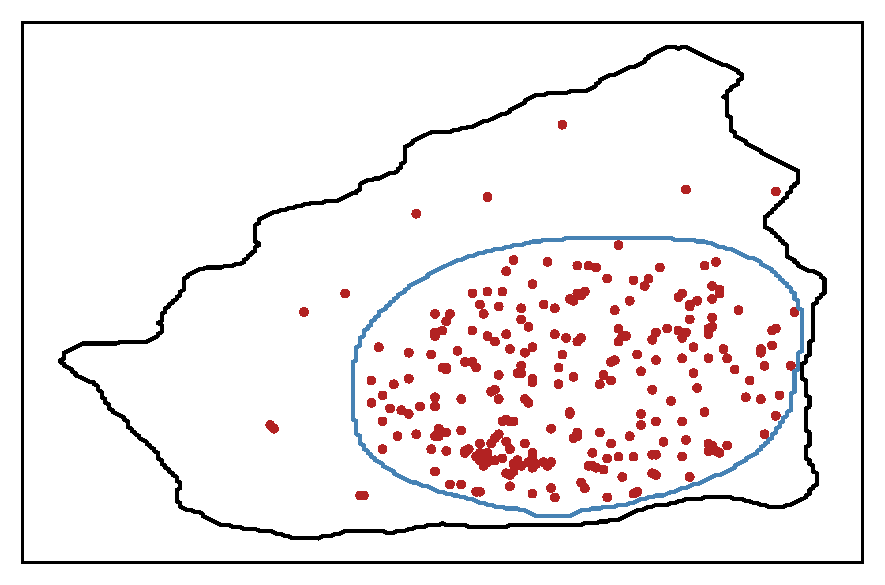
\includegraphics[trim={0.5cm 0.5cm 0.5cm 0.5cm},clip,width=\linewidth]{figures/chapter5/plot_intranuclear}
		\subcaption{Intranuclear}
	\endminipage\hfill
	\minipage{0.2\textwidth}
		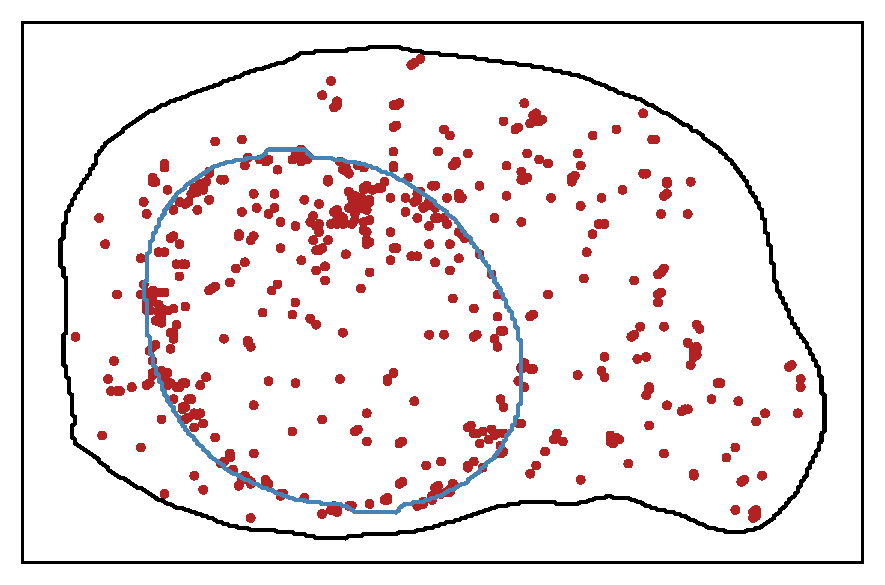
\includegraphics[trim={0.5cm 0.5cm 0.5cm 0.5cm},clip,width=\linewidth]{figures/chapter5/plot_nuclear}
		\subcaption{Nuclear edge}
	\endminipage\hfill
	\minipage{0.2\textwidth}
		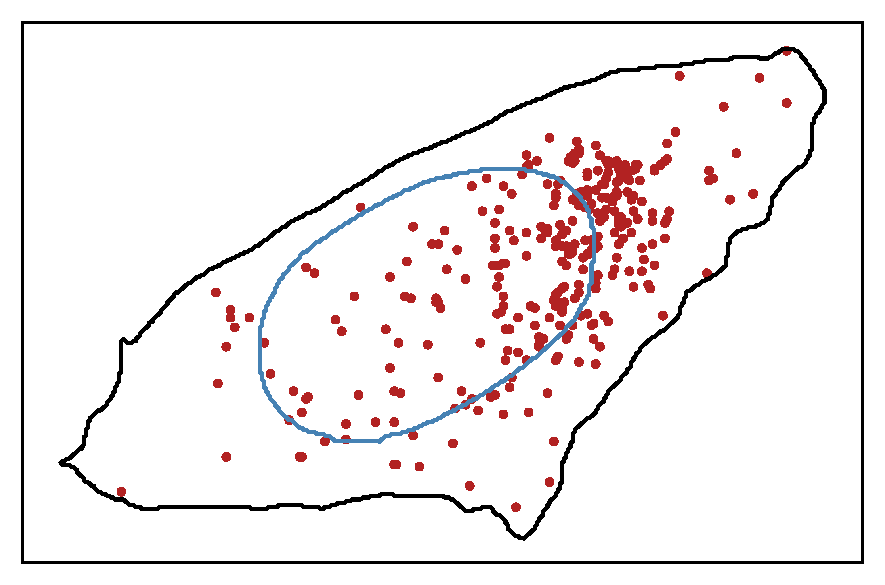
\includegraphics[trim={0.5cm 0.5cm 0.5cm 0.5cm},clip,width=\linewidth]{figures/chapter5/plot_perinuclear}
		\subcaption{Perinuclear}
	\endminipage\hfill
	\minipage{0.2\textwidth}
		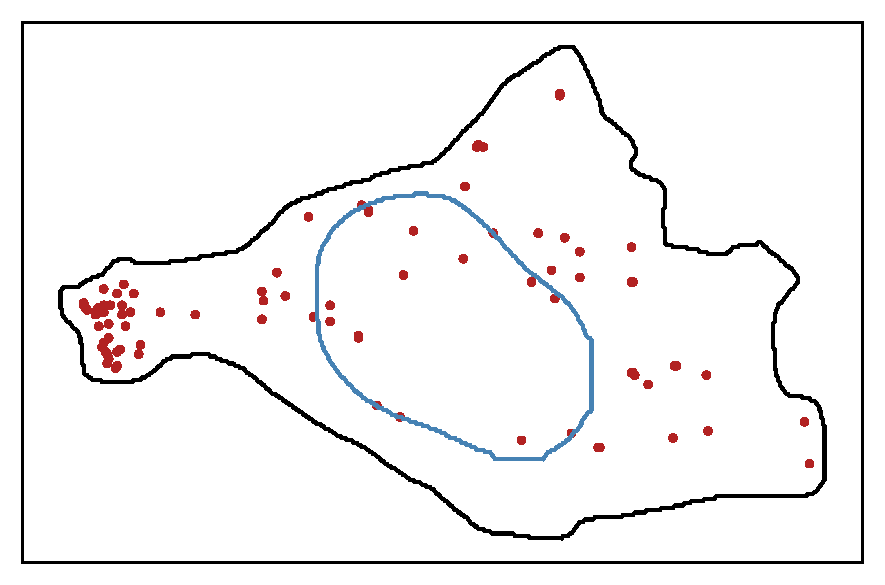
\includegraphics[trim={0.5cm 0.5cm 0.5cm 0.5cm},clip,width=\linewidth]{figures/chapter5/plot_protrusion}
		\subcaption{Protrusion}
	\endminipage
	\caption{RNA localization patterns from~\cite{CHOUAIB_2020}.
	Coordinate representations with RNA spots (\textit{red}), cell membrane (\textit{black}) and nuclear membrane (\textit{blue}).
	Detection and segmentation results are extracted and visualized with \emph{bigfish}}
	\label{fig:localization_patterns_racha_features}
\end{figure}

I use these hand-crafted features to train several binary classifiers, one for each localization pattern we want to recognize.
Five specific localization patterns are defined - foci, intranuclear, nuclear edge, perinuclear, protrusion - and the random pattern is considered as a default one.
Figure~\ref{fig:localization_patterns_racha_features} illustrates an example of these patterns with a coordinate representation.

To train the classifiers, manual annotations are needed as a ground truth.
I generate panels with the cropped original image of the individual cells and their coordinate representations.
These panels are then manually tag with the appropriate localization pattern.
The manual classification result has been independently checked by several trained microscopists.
Ultimately, I end up with 810 annotated cells.
Counts of the annotations are presented in Table~\ref{table:real_dataset_chapter5}.

\begin{wraptable}{L}{0.50\textwidth}
	\centering
	\begin{tabular}{| c | c |}
		\hline
		Pattern & \# of cells \\
		\hline
		Random & 372\\
		Foci & 198\\
		Intranuclear & 73\\
		Nuclear edge & 87\\
		Perinuclear & 64\\
		Protrusion & 83\\
		\hline
	\end{tabular}
	\caption{Annotated cells}
	\label{table:real_dataset_chapter5}
\end{wraptable}

One way to evaluate how relevant is the feature space is to investigate the distribution of the annotated cells within it.
To do so, I reduce the dimensionality with a \ac{t-SNE} transformation~\cite{vandermaaten_2008} in order to visualize the features point cloud.
From the multi-dimensional feature space, I obtain a 2D vector representation I can plot.
In term of setting, I initialize the \ac{t-SNE} with a PCA transformation first and use a perplexity value of 30.

I also define a supervised learning problem with the training of 5 independent binary Random Forest classifiers~\cite{breiman_random_2001}.
The choice to design the problem as several binary ones instead of one multi-class problem allows me to define the localization patterns as non mutually exclusives.
Indeed, an individual cell can display several patterns at the same time, like \ac{RNA} clusters (foci) localizing around the nuclear membrane (nuclear edge).
For each model, I build a training set including all the cells of one class and a subsampling of cells from others classes, such that the imbalance is 1:4 for the positive class.
This is a ''one vs.\ all'' training strategy.
Eventually, I exploit the \ac{OOB} error allowed by the random forest design.
In such manner, the model can ''be fit in one sequence, with cross-validation being performed along the way.''~\cite{hastie_elements_2009}.
Random forest is an ensemble model of tree classifiers.
Each tree is trained on a subsample of the observations and a subset of features.
This ensembling framework makes random forest quite robust to overfitting.
For every sample, an \ac{OOB} prediction can be computed using only the trees fitted without the sample.
I initialize the random forests with 100 trees, a maximal depth of 3 and a minimum number of samples per splitter node of 2.
During the training, for each split, I consider a subset of 10 features and entropy criterion.
In addition, input dataset is rescaled to have zero mean and unit variance.

\subsection{Results}
\label{subsec:results_general_pattern}

Thanks to their design or their normalization, the spatial features selected are mostly invariant to \ac{RNA} concentration.
They allow the use of unsupervised or supervised methods to classify cells among several localization patterns.

\subsubsection{Unsupervised visualization}

\begin{figure}[]
    \centering
    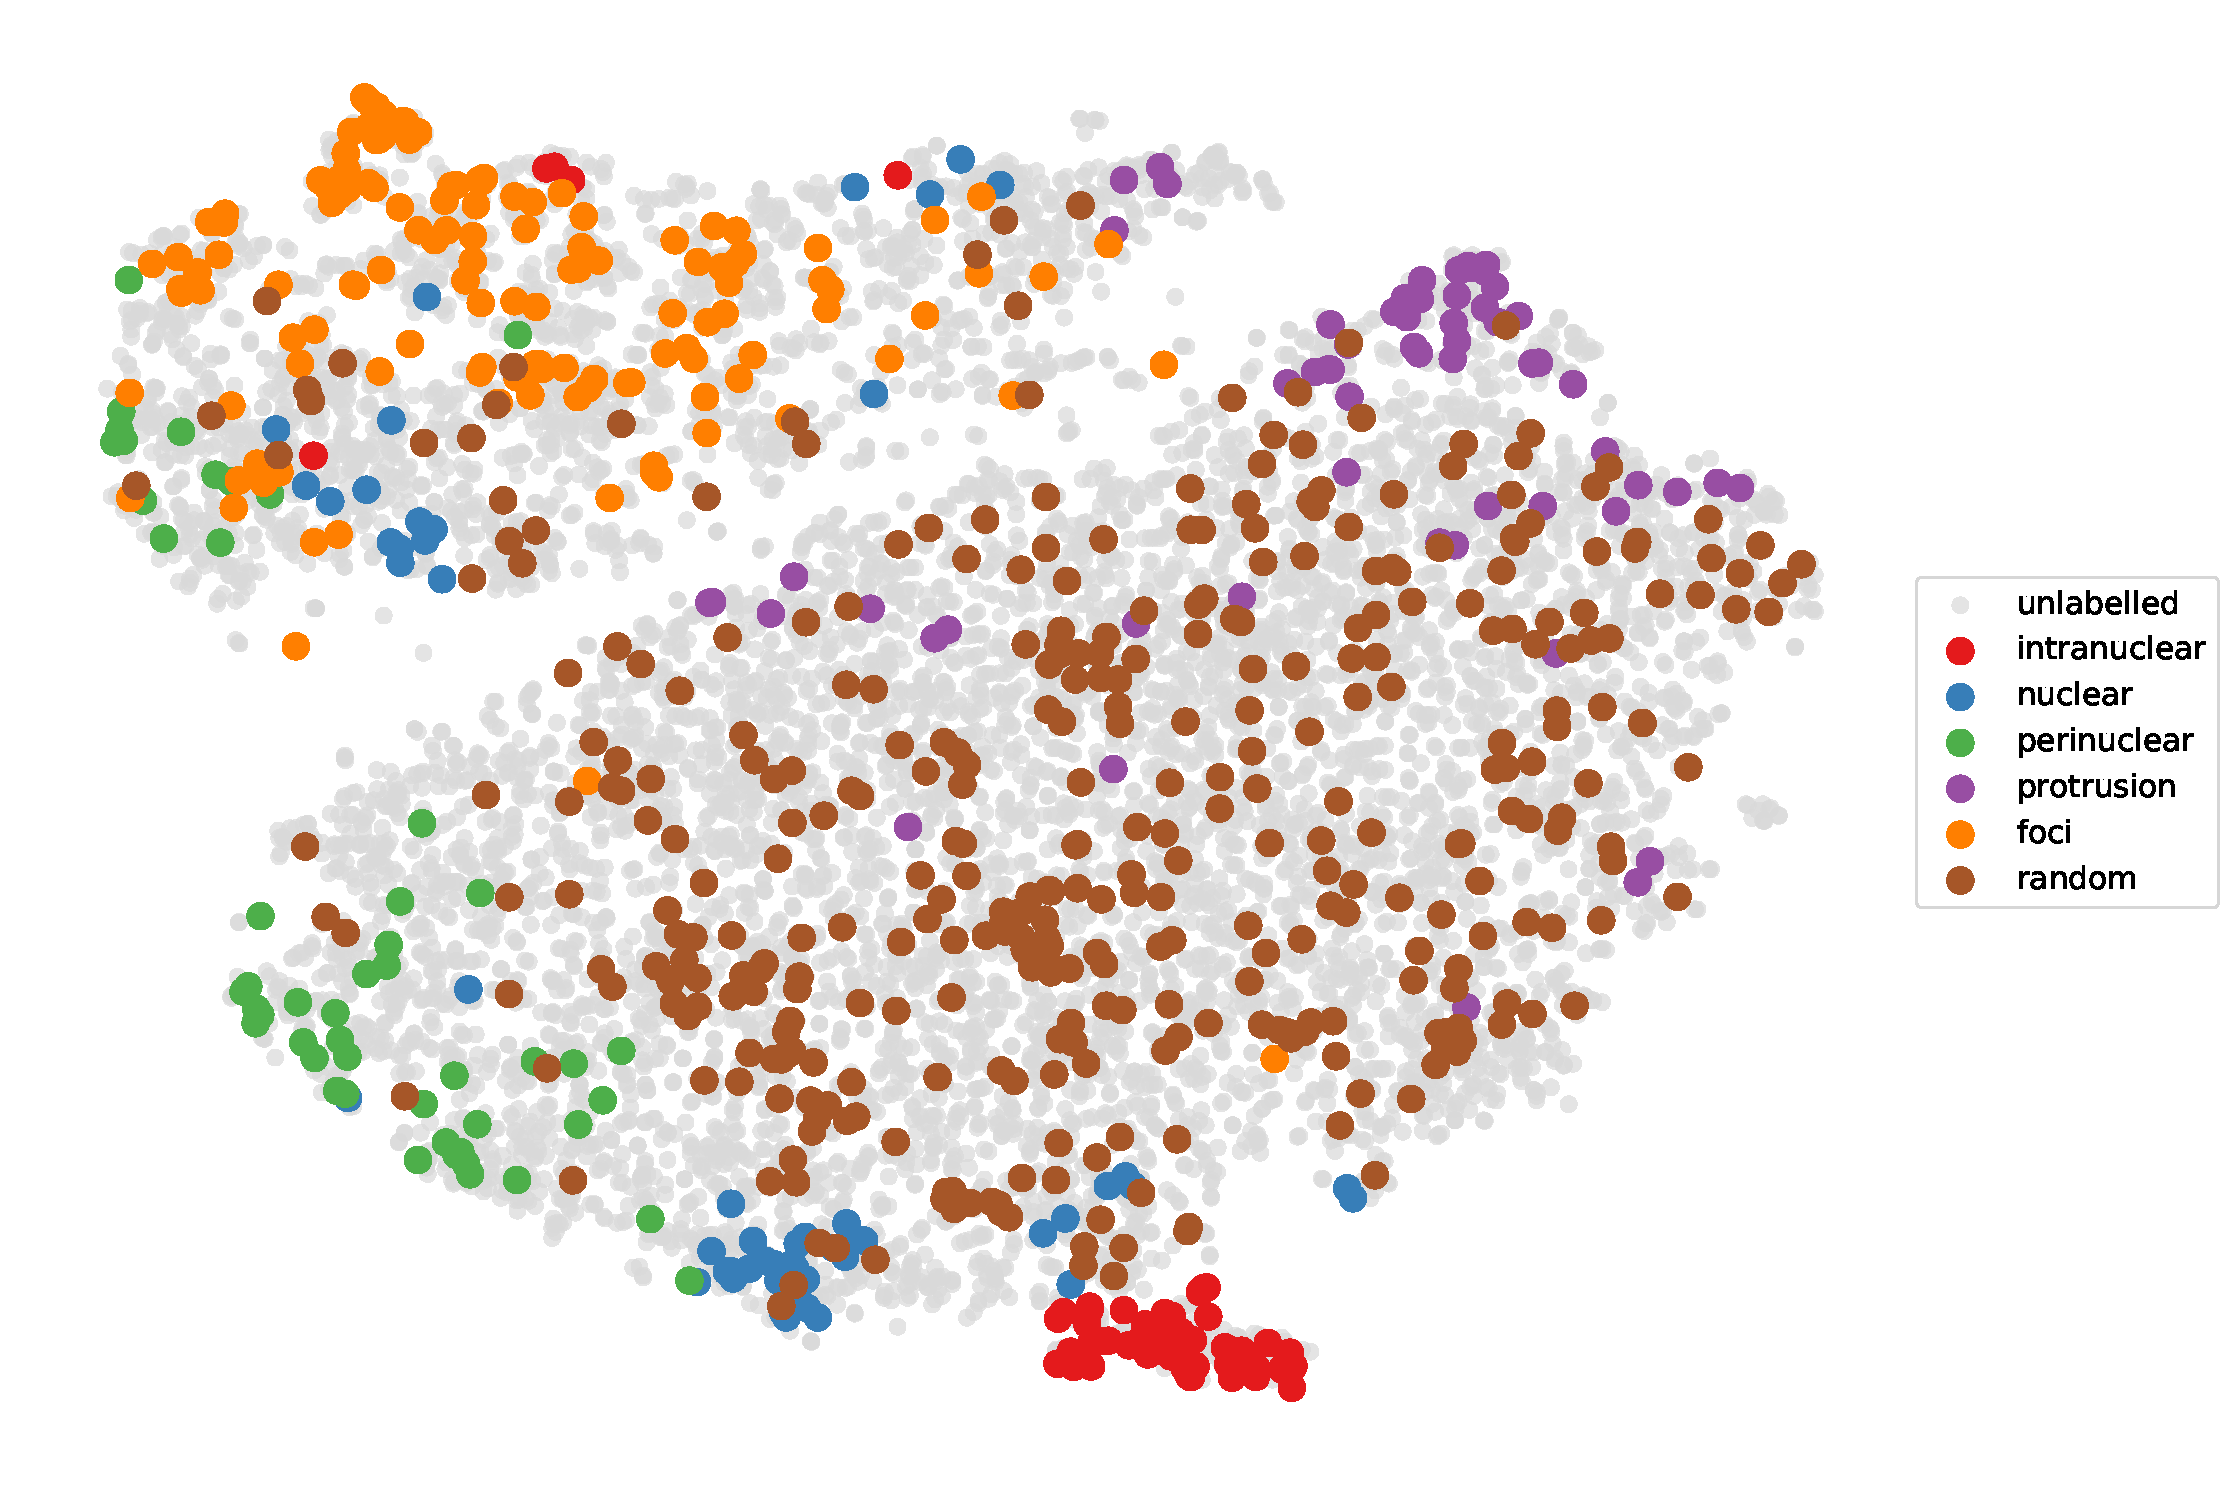
\includegraphics[width=\textwidth]{figures/chapter5/tsne_annotation_legend}
    \caption{t-SNE embedding from~\cite{CHOUAIB_2020}.
	Each point is a cell in the feature space after a t-SNE transformation.
	Manually annotated cells are colored according to their localization pattern.
	Cells that were not annotated or that had multiple patterns are colored in gray}
    \label{fig:tsne_annotation_racha}
\end{figure}

The resulting embedding from the \ac{t-SNE} algorithm can be observed in Figure~\ref{fig:tsne_annotation_racha}.
Cells with different patterns are localized in different regions of the embedded feature space.
Moreover, cells with the same annotations cluster in the same regions whether they correspond to the same gene or not.
With these observations it seems the hand-crafted features capture key information of the localization patterns and summarize well the manual annotations.

Initialized with a PCA transformation, a \ac{t-SNE} algorithm preserves better the global structure, thus allowing more relevant global interpretation.
In particular, we can discriminate on the top a large cluster of cells with a potential foci pattern from the rest of the cell population.
The resulting embedding also seems to polarize between nucleus-related patterns (bottom left) and the cell-related patterns (top right).
This polarization remains even among the subpopulation with potential foci pattern.
Such conclusion validates the design to let a cell being classified with several non-exclusive localization patterns.
Indeed, a foci can be localized in a relevant subcellular compartment.

\subsubsection{Gene aggregated classifications}

Not surprisingly, a feature space that discriminates well between classes also performs well when fed into a robust random forest classifier.
The \ac{OOB} accuracy score obtained for the different patterns is between 0.93 and 0.99, while a dummy classifier would return a 0.8 accuracy score (the dataset is built with 20\% positive samples).
The intranuclear pattern is the easiest to recognize.
In fact, it could be predicted by just thresholding the proportion of \ac{RNA} inside nucleus (almost all intranuclear cells have more than 80\% of their\ac{RNA}s that localize inside the nucleus).
On the opposite, the nuclear edge and perinuclear patterns are the most difficult to classify due to possible confusion with a random pattern or the lake of annotated cells.

\begin{wraptable}{R}{0.50\textwidth}
	\centering
	\begin{tabular}{| c | c |}
		\hline
		Pattern & Accuracy score\\
		\hline
		Random & -\\
		Foci & 0.95\\
		Intranuclear & 0.99\\
		Nuclear edge & 0.93\\
		Perinuclear & 0.93\\
		Protrusion & 0.94\\
		\hline
		\textit{Dummy classifier} & \textit{0.80}\\
		\hline
	\end{tabular}
	\caption{Random forest accuracy (OOB)}
	\label{table:accuracy_oob}
\end{wraptable}

For each cell, I can compute 5 binary predictions, one per pattern.
Individual cell is assigned to a pattern if the probability given by the random forest classifier for that pattern is higher than 0.5.
If no pattern is detected, cell is classified with a random localization pattern.
In total, I analyze 27 different genes through a population of 9,710 cells, with only one kind of transcript being targeted per cell.
The number of cells identified per gene varies, thus predictions are aggregated at the gene level.
This aggregation also facilitates the validation of biological insights and helps understanding the mechanism at stake for specific group of genes.
For every gene, I compute the proportion of cells displaying each indicated localization pattern.
Results are eventually reported in a heat map~\ref{fig:heatmap_racha}, for every gene and pattern.
Importantly, row values does not sum to one because classifiers (and so columns predictions) are independent.

\begin{figure}[]
    \centering
    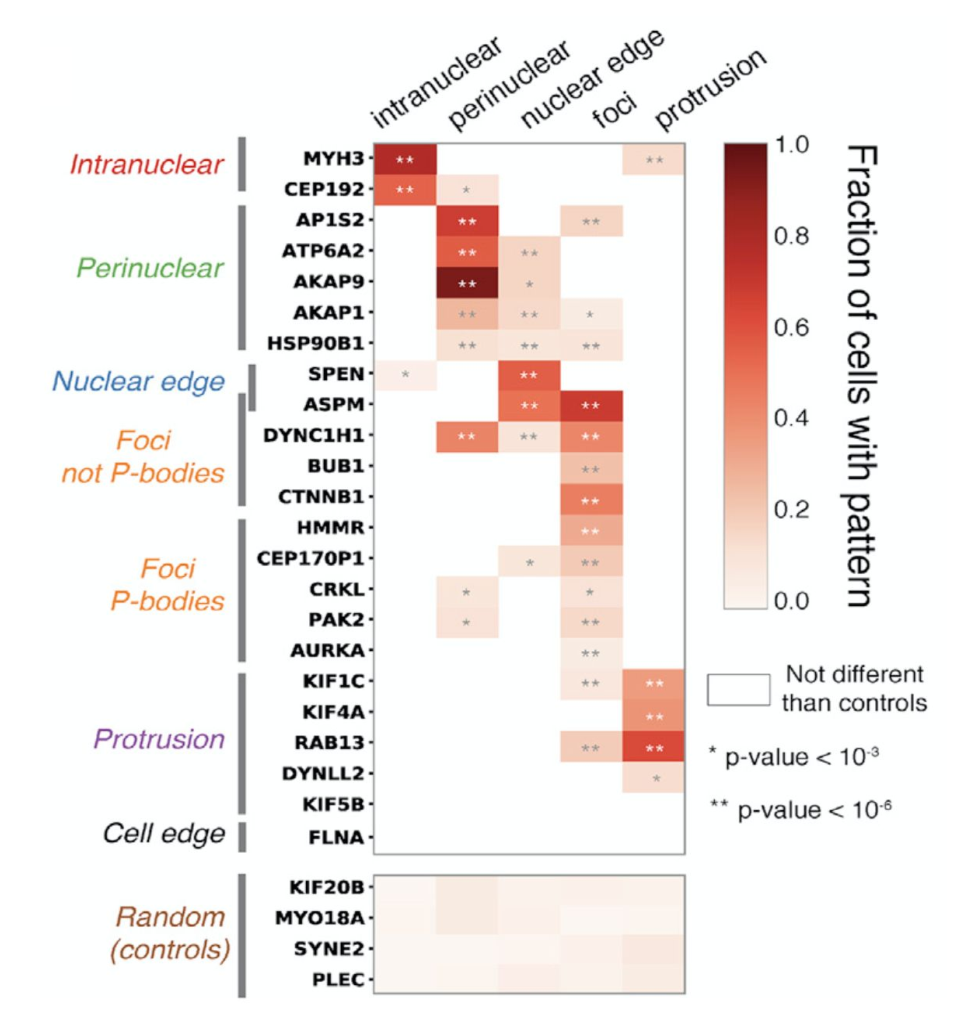
\includegraphics[width=\textwidth]{figures/chapter5/heatmap_racha_2}
    \caption{Heat maps from~\cite{CHOUAIB_2020} with the fraction of cells classified in the indicated pattern.
	(\textit{Top heat map}) Genes whose RNAs shows a localization preference.
	Only values significantly different from negative controls are colored (p-value computed with Fisher's exact test).
	(\textit{Bottom heat map}) Negative control with genes whose RNAs localize randomly.
	(\textit{Left bars}) Manual annotations of the genes are indicated with the same color scheme than Figure~\ref{fig:tsne_annotation_racha}}
    \label{fig:heatmap_racha}
\end{figure}

We manually identify a group of random genes that can be used as a control group: KIF20B, MYO18A, SYNE2 and PLEC.
Therefore, it is possible to perform statistical testing over the aggregated predictions.
A Fisher's exact test can measure if the proportion of cells observed with a pattern is significantly greater than the proportion observed in the control group (with a $\text{p-value} < 10^{-3}$).
Genes whose transcripts present a significant localization preference are reported in Figure~\ref{fig:heatmap_racha}.

Overall, we observe consistent results with the manual annotations performed by the biologists (the colored annotations in the \ac{t-SNE} plot~\ref{fig:tsne_annotation_racha} and the vertical colored bars next to the heat map~\ref{fig:heatmap_racha}).
The agreement between automated and manual classification holds with a high degree of statistical significance, except for FLNA and KIF5B.
FLNA transcripts are manually identified with a potential cell edge pattern.
However, such localization is difficult to recognize with the quantitative pipeline, mostly because the pattern is visible in 3D while my cell segmentation, and the spatial features resulting from it, is in 2D.
For these reason we do not study in depth this localization pattern.

\subsubsection{Recognition of five localization patterns}

Apart from KIF5B, others transcripts localizing in cytoplasmic extensions (or protrusions) are correctly identified: KIF1C, KIF4A, RAB13 and DYNLL2.
The frequency of this pattern varies a lot, between 14\% and 62\% of cells classified, respectively for DYNLL2 and RAB13.
Interestingly, this pattern concerns four \ac{RNA}s encoding motor proteins: the three kinesins KIF1C, KIF4A, KIF5B and DYNLL2.

MYH3, another transcript encoding motor protein, localizes partially in protrusions, although it's not its most frequent localization pattern.
Most of the time, MYH3 transcripts remain in the nucleus, exhibiting an intranuclear pattern.
This is the most easily recognizable pattern: more than 55\% of cells spotting MYH3 and CEP192 \ac{RNA}s show an accumulation of transcripts inside nucleus.

The two genes observed with a nuclear edge pattern, ASPM and SPEN, have 50\% and 55\% of cells identified with this localization, respectively.

Several genes are identified with \ac{RNA}s in the perinuclear area: AKAP1, AKAP9, AP1S2, ATP6A2, and HSP90B1.
They ranged from 13\% (HSP90B1) to 93\% (AKAP9) of cells classify with said pattern.
Even with a small number of cells HSP90B1 shows a significant perinuclear pattern compare to the control group.
Such observation is consistent with previous biological information about this gene: it contains a signal peptide that leads the translation (and the subsequent protein) on the endoplasmic reticulum, resulting in a perinuclear pattern through a 2D \ac{smFISH} experiment.
This also suggests that HSP90B1 transcript co-localizes with its protein.

A large number of transcripts exhibit a cluster-like localization pattern we call foci.
We classify them in two groups we detail in the next Section~\ref{sec:translation_factories}.
The first group gathers transcripts accumulating in \ac{P-bodies}: AURKA, HMMR, CEP170P1, CRKL and PAK2.
The second group includes ASPM, DYNC1H1, BUB1 and CTNNB1 transcripts, accumulating in non-\ac{P-bodies} clusters we call translation factories.
It is noteworthy to mention that a number of genes exhibit foci with another localization preference in parallel like ASPM (nuclear edge), DYNC1H1, AP1S2, AKAP1, HSP90B1 (perinuclear), KIF1C and RAB13 (protrusion).
In general, non-\ac{P-bodies} genes have a higher proportion of cells classified with a foci pattern: between 24\% (BUB1) and 69\% (ASPM) cells while \ac{P-bodies} genes have between 7\% (AURKA) and 31\% (HMMR) cells.
Likewise, in term of molecule concentration, non-\ac{P-bodies} genes present a higher proportion of \ac{mRNA} in foci, varying from 9\% (BUB1) to 28\% (CTNNB1), while \ac{P-bodies} accumulate between 2\% to 15\% of cell \ac{mRNA}s.
This foci quantification is in line with the previously reported estimations in the literature of 10\% to 20\% \ac{mRNA}s clustered in foci~\cite{Pillai_2005, Hubstenberger_2017}.

\subsubsection{Cell-to-cell variability}

If we focus on the individual cells instead of the gene, \ac{RNA} localization appears highly variable.
For example, with CTNNB1 transcripts there is no foci at all or more than 60\% of \ac{mRNA}s clustered, depending of the cell observed.
For a better quantification of this intercellular variability, additional figures are presented in Appendix~\ref{ch:cell_pattern_classification}.
Cells of specific genes are plotted on \ac{t-SNE}~\ref{fig:tsne_proba_gene} and single cell results are summarized in heat maps~\ref{fig:heatmap_racha_cells}.
Pattern probabilities returned by classification models vary from cell to cell.
For a given gene, cells are dispersed on the \ac{t-SNE} plot, although a majority of them still accumulate in the expected area.
Finally, some cells have several localization patterns simultaneously.
As listed before, it the case for the cells with localized \ac{RNA} clusters, combining a foci pattern with a protrusion or a nucleus-related pattern.
Likewise, MYH3 cells frequently show an intranuclear and protrusion pattern.

In conclusion, my quantitative pipeline corroborates the manual observations and measures a high degree of heterogeneity of \ac{RNA} localization across different cells.
This variability is a general phenomenon, at least for HeLa cells, since it is seen with nearly all the genes analyzed in~\cite{CHOUAIB_2020}.
In comparison, \ac{RNA} localization in embryos appears to be much more stereotyped.

\section{The case for translation factories}
\label{sec:translation_factories}

Beyond the generic pattern recognition pipeline I have implemented, another important quantitative result concerns the characterization of a cluster-like localization pattern we name \emph{translation factory}.
This analysis is part of a broader investigation about the co-localization of \ac{mRNA}s and their encoded proteins, a major contribution of~\cite{CHOUAIB_2020}

\subsection{Introduction}
\label{subsec:introduction_translation_factories}

Studies previously mentioned focus on \ac{RNA} localization, but do not detect translated proteins~\cite{lecuyer_global_2007, battich_image-based_2013, Chen_2015, eng_seqfish_2019, Xia_2019}.
This makes impossible a complete analysis of the local translation mechanisms and their functions.
In~\cite{CHOUAIB_2020}, we performed a high-content screen in HeLa cells and visualize simultaneously the \ac{mRNA} and its encoded protein.
More precisely, we exploit a library of HeLa cell lines with a \ac{BAC} including a \ac{GFP}-tagged gene~\cite{poser_bac_2008} in order to visualize the selected proteins.
In parallel, and without compromising the localization of the \ac{mRNA}, the tag can be targeted with a \ac{smFISH} probe, allowing us to spot the \ac{mRNA} molecules.

Along with \ac{RNA} localization patterns, we observe occurrences of local translation in several subcellular areas.
Some are expected, like HSP90B1 (an endoplasmic reticulum protein), ATP6A2 (in endolysosomes) or AKAP1 (an \ac{RBP} at the surface of mitochondria).
Others are discoveries like AKAP9 or AP1S2, whose \ac{mRNA}s are known to localized respectively in the Golgi or on endosomes.
For example the phenomenon is observed in the nuclear membrane with the ASPM and SPEN transcripts.
Previous studies have exploited SunTag to visualize single molecules of nascent proteins~\cite{pichon_visualization_2016, Pichon_2018, Wu_2016}.
Here, this techniques allows us to confirm that both ASPM \ac{mRNA}s and nascent proteins localized in nuclear membrane, thus supporting a local translation.
Additionally, we find that these transcripts localize through translation-dependent mechanisms related to the nascent peptide: by blocking the translation and releasing the polysome complex the localization pattern disappears.

The rest of this section focuses on foci pattern where we discriminate another translation-dependent cluster-like pattern from the more common \ac{P-bodies}.
We find four transcripts that accumulate in clusters, but do not colocalized with \ac{P-bodies} markers: BUB1, DYNC1H1, CTNNB1 and ASPM.
We name such complex \emph{translation factory}, where specific \ac{mRNA}s accumulate to be translated, and not repressed.
Indeed, we observe in these clusters a co-concentration of \ac{RNA} with nascent proteins, like in Figure~\ref{fig:translation_factory}.
Finally, my second contribution to~\cite{CHOUAIB_2020} consists in quantify this unexpected phenomenon, exploiting my cluster detections methods and experiments with a translation inhibition protocol.

\begin{figure}[]
    \centering
    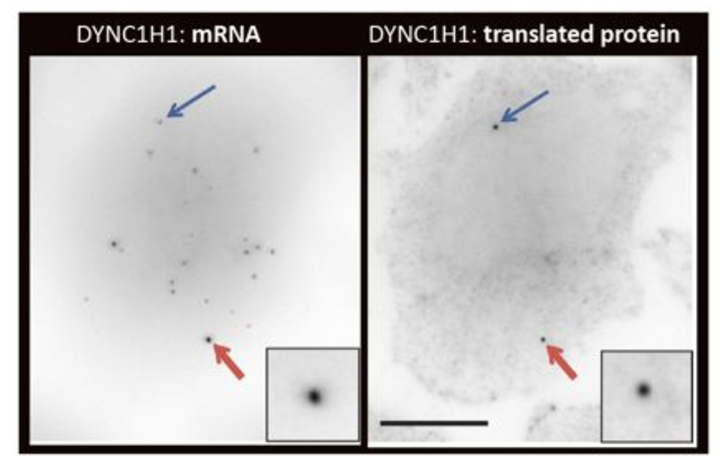
\includegraphics[width=\textwidth]{figures/chapter5/translation_factory}
    \caption{Colocalization between the DYNC1H1 transcript and its nascent protein, from~\cite{pichon_visualization_2016}.
	Transcripts and proteins are targeted with smFISH probes (\textit{Left}) and SunTag (\textit{Right}) respectively.
	\textit{Scale bar} is 10$\mu$m}
    \label{fig:translation_factory}
\end{figure}

\subsection{Materials and methods}
\label{subsec:materials_translation_factories}

In the continuation of the contribution presented in Section~\ref{sec:general_pattern_recognition}, this work is developed in Python and available online\footnote{\url{https://github.com/Henley13/paper_translation_factories_2020}}.

\subsubsection{Puromycin drug}

The use of puromycin drug inhibits translation by inducing early termination and releasing the nascent peptide chain from the ribosomes.
On the opposite, a cycloheximide treatment inhibits translation by freezing the ribosomes on the \ac{mRNA}s.

indicating that their localization did not require protein
% synthesis per se, but more likely the presence of nascent proteins on polysomes.

% paper Racha (puromycin vs cycloheximide)

% To distinguish between these possibilities, we inhibited either transcription with actinomycin D, or translation with puromycin. After 1 h of
% actinomycin D treatment, SPEN and ASPM mRNAs still localized at the nuclear envelope (left panels in Figures 4A, S9C, and
% 4B for quantifications). On the contrary, both mRNAs became dispersed after 1-h exposure to puromycin (Figures 4A, 4B, S9C,
% and S10A for quantifica- tions). We then used cycloheximide, which inhibits translation by freezing the ribosomes on the mRNAs,
% in contrast to puromy- cin that induces premature termination and releases the nascent peptide. Cycloheximide had no effects
% on the localization of ASPM mRNAs (Figures 4A left panels and 4B), indicating that their localization did not require protein
% synthesis per se, but more likely the presence of nascent proteins on polysomes. Therefore, ASPM and SPEN mRNAs at the nuclear
% envelope are not in transit to the cytoplasm but localize on the nuclear en- velope by a translation-dependent mechanism requiring the nascent protein.


% racha paper (use of puromycin)

% Translation Inhibition with Puromycin Frequently Prevents mRNA Localization

% Since the localization of ASPM mRNA at the envelope is translation dependent, we tested whether this was also the case for its
% localization at centrosomes. Puromycin abolished its localiza- tion, while actinomycin D and cycloheximide had little effect
% (Fig- ure 4A, right panels; Figure 4B for quantification). The effect of puromycin was then tested on the other localized mRNAs.
% After 1 h of treatment, KIF1C and MYH3 mRNAs still localized to cyto- plasmic protrusions (Figures 5A and 5B for quantifications).
% In contrast, HSP90B1, HMMR, AP1S2, AKAP1, KIF4A, and AKAP9 mRNAs all became delocalized and lost co-localization with their
% ncoded protein when translation was inhibited (Fig- ures 5C–5E and S10A–S10D). The data demonstrated are consistent with the
% hypothesis that translation is required for the localization of these mRNAs.

% racha paper (translation factories)

% Non-P-Body mRNA Foci Correspond to Specialized Translation Factories
% Four mRNAs accumulated in foci that were distinct from P- bodies (BUB1, DYNC1H1, CTNNB1/b-catenin, and ASPM; Fig- ure S6A).
% The dynein heavy-chain DYNC1H1 and the ASPM pro- tein were described above. BUB1 is a checkpoint kinase that
% verifies the attachment of microtubules to kinetochores at the onset of mitosis (Saurin, 2018), and b-catenin is the
% key tran- scription factor of the Wnt signaling pathway (Grainger and Wil- lert, 2018). SmiFISH confirmed that the four
% endogenous mRNAs accumulated in foci (Figures S2A, S8C, S10E, and see below S11F). Moreover, dual-color smiFISH showed
% that these foci did not co-localize together, indicating that they were distinct structures (Figure 6A).
% We then inhibited translation with puro- mycin, using an mRNA accumulating in P-bodies as control (AURKA).
% After 1 h of treatment, the non-P-body foci virtually dis- appeared (Figures 6B and 6C), while the accumulation
% of AURKA mRNA in P-bodies actually increased. Thus, translation inhibition specifically disrupted the mRNA foci
% that were not P-bodies. We previously used the SunTag to show that DYNC1H1 is translated in the mRNA foci (Pichon et al., 2016).
% Using the CRISPR SunTag clone described above, we found that ASPM mRNAs were simi- larly translated in the mRNA foci
% (Figure 4C, orange arrow; 70\% of the foci have a SunTag signal). A 32xSunTag repeat was then introduced at the N terminus of the BUB1
% protein using CRISPR gene editing. BUB1 mRNAs were detected by smiFISH and were found to be frequently translated in the foci
% (Figures 6D and 6E; 70\% of the foci contained a SunTag signal), in contrast to mRNAs located outside foci for which the SunTag signal was
% rarely detected (1\% of the time). Taken together, these data demonstrated that ASPM, BUB1, and DYNC1H1 are translated
% in mRNA foci, which thus correspond to specialized translation factories.

%%%%%%%%%%%%%%%%%%%%%%%%%%%%%%%%%%%%%%%%%%%%%%%%%%%%%%%%%%%%%%%%%%%%%%%%%%%%%%%%%%%%%%%%

% paper Racha (puromycin vs cycloheximide)

% To distinguish between these possibilities, we inhibited either transcription with actinomycin D, or translation with puromycin. After 1 h of
% actinomycin D treatment, SPEN and ASPM mRNAs still localized at the nuclear envelope (left panels in Figures 4A, S9C, and
% 4B for quantifications). On the contrary, both mRNAs became dispersed after 1-h exposure to puromycin (Figures 4A, 4B, S9C,
% and S10A for quantifica- tions). We then used cycloheximide, which inhibits translation by freezing the ribosomes on the mRNAs,
% in contrast to puromy- cin that induces premature termination and releases the nascent peptide. Cycloheximide had no effects
% on the localization of ASPM mRNAs (Figures 4A left panels and 4B), indicating that their localization did not require protein
% synthesis per se, but more likely the presence of nascent proteins on polysomes. Therefore, ASPM and SPEN mRNAs at the nuclear
% envelope are not in transit to the cytoplasm but localize on the nuclear en- velope by a translation-dependent mechanism requiring the nascent protein.

% paper Racha

% To measure the degree of spatial overlap between mRNA (by smFISH) and protein
% (by the GFP fluorescence), we calculated an enrichment ratio. Cells and nuclei
% were outlined manually in 2D based on the GFP and DAPI image, respectively.
% The subsequent analysis was restricted to the cytoplasm. FISH-quant was used
% to detect mRNAs in 3D and each cell was post-processed separately.
% First, we calculated the median pixel intensity in the GFP image at the identified RNA positions.
% Second, we estimated a normalization factor as the median GFP intensity of the outlined cytoplasm within the z-range of the detected mRNAs.
% The enrichment ratio was then estimated as the ratio of the median GFP intensity at the RNA positions divided by the mean cytoplasmic GFP intensity.

%%%%%%%%%%%%%%%%%%%%%%%%%%%%%%%%%%%%%%%%%%%%%%%%%%%%%%%%%%%%%%%%%%%%%%%%%%%%%%%%%%%%%%%%

\subsubsection{Cluster detection}

Both on the treated and untreated cells I re-apply my spot detection algorithms, the decomposition of dense areas with large agglomeration of spots and ultimately the detection of \ac{RNA} clusters, directly from their detected coordinates (see Subsection~\ref{subsec:materials_general_pattern}).
It is important to note that the cluster detection is distinct from the dense area decomposition.
Such areas can be processed in a way that no cluster is detected afterward.

\subsection{Results}
\label{subsec:results_translation_factories}

% CTNNB1 gene encoding for β-catenin protein

\begin{center}
	\textit{(To be completed)}
\end{center}

\begin{figure}[]
    \centering
    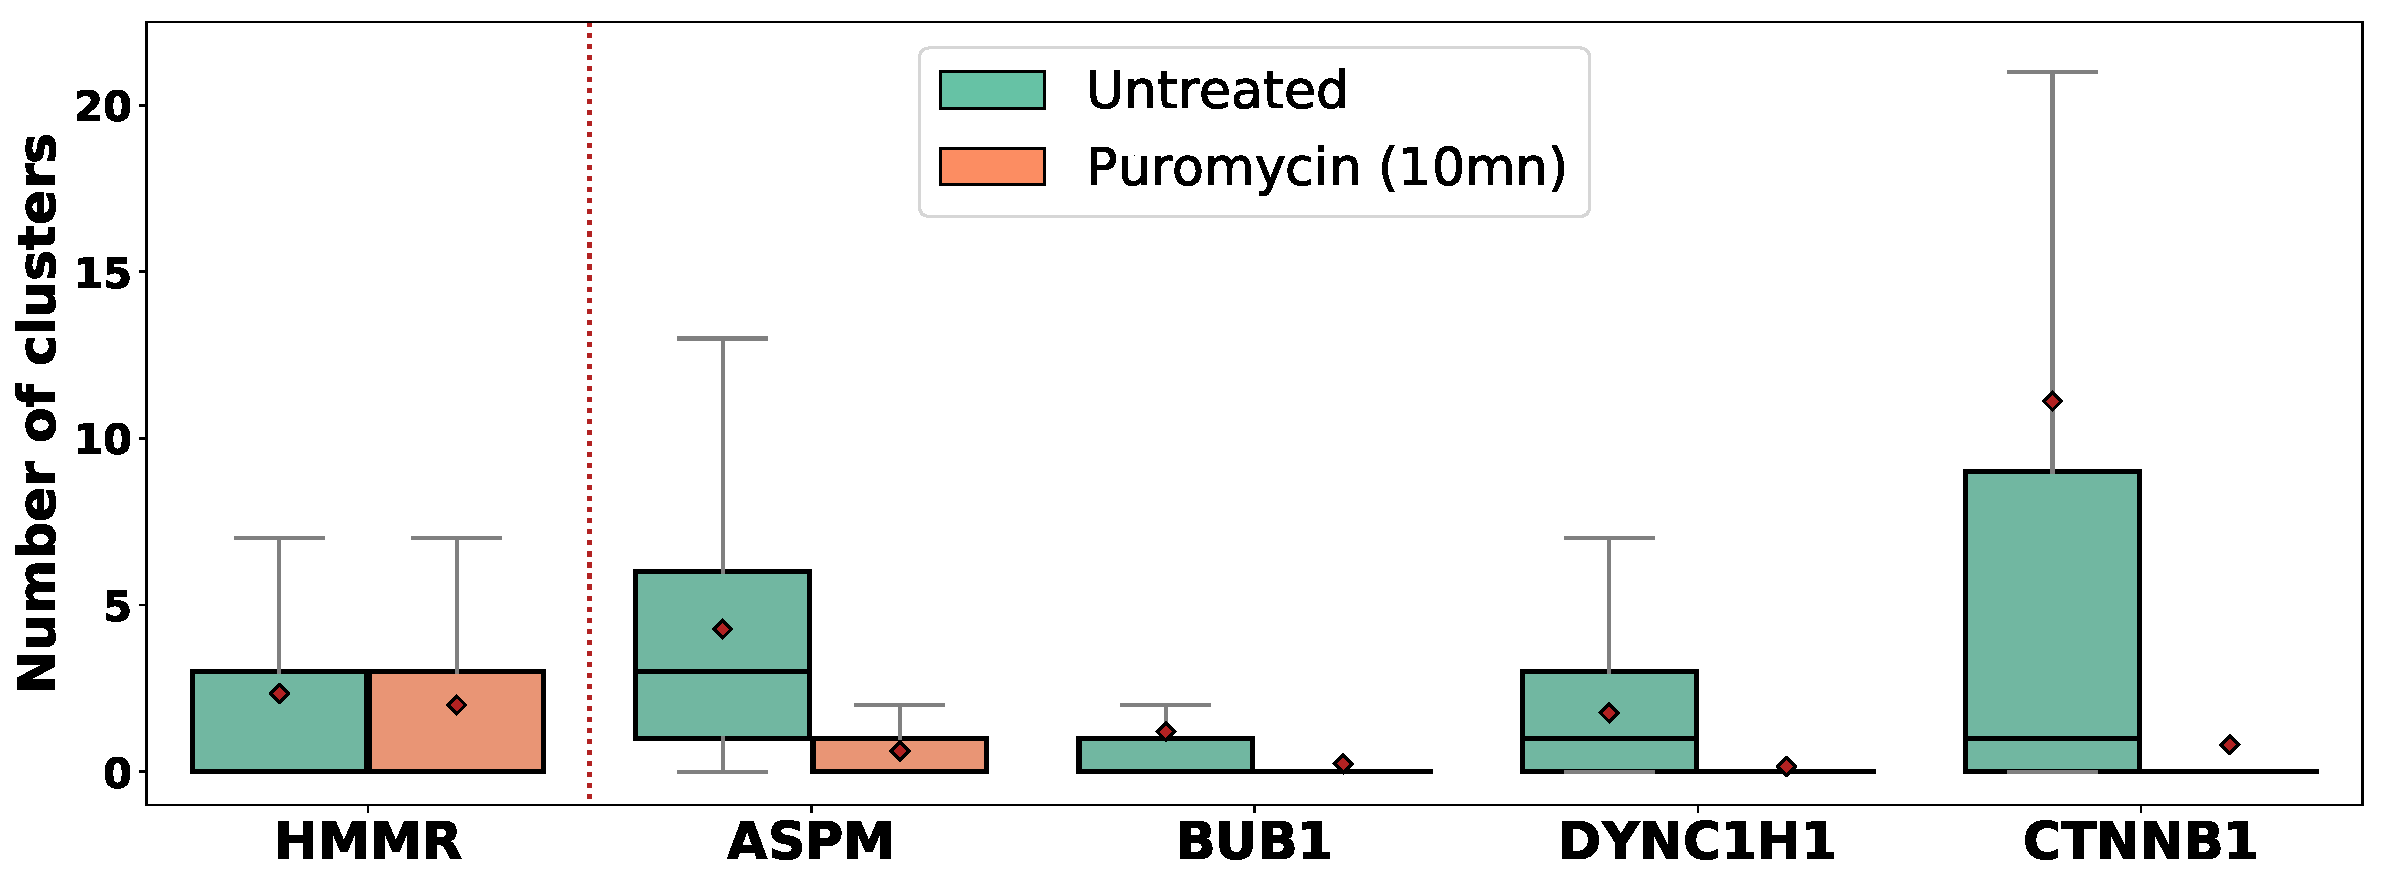
\includegraphics[width=\textwidth]{figures/chapter5/plot_puromycin}
    \caption{Impact of treatment with translational inhibitor puromycin on the number of detected RNA clusters}
    \label{fig:plot_puromycin}
\end{figure}

% 1) descriptin of the plot
% 2) the case for CTNNB1

%%%%%%%%%%%%%%%%%%%%%%%%%%%%%%%%%%%%%%%%%%%%%%%%%%%%%%%%%%%%%%%%%%%%%%%%%%%%%%%%%%%%%%%%

% paper fq2
% HMMR shows a similar number of clusters, while all other genes have significantly fewer, indicating an implication of translation in cluster formation.

% paper racha

% For the pattern ‘‘foci,’’ the non-P-body genes (ASPM, BUB1, CTNNB1, and DYNC1H1)
% had a high proportion of cells classified in that pattern (24% for BUB1 and up to 69% for ASPM)
% and an average proportion of mRNA in foci varying from 9% (BUB1) to 28% (CTNNB1; Figure S6B).
% In contrast, the mRNAs accumulating in P-bodies had a comparatively smaller fraction of
% cells classi- fied in the ‘‘foci’’ pattern (7% to 31%), as well as a smaller frac- tion
% of the mRNAs in foci (2% to 15%). Note that our estimation of the fraction of mRNA in
% foci correspond to a lower bound because we only counted groups of molecules where each molecule was closer than 350 nm to the group, while foci can be larger.
% Nevertheless, and taking into account our stringent cri- terion, our quantification was in the
% lower range of previously re- ported quantifications of P-body mRNAs (10%–20% of the total mRNAs; Pillai et al., 2005; Hubstenberger et al., 2017).
% When comparing individual cells, the quantifications indicated that RNA localization
% can be highly variable even for the same mRNA. For instance, the fraction of CTNNB1 mRNA
% in foci varied from 0% to more than 60%.

%%%%%%%%%%%%%%%%%%%%%%%%%%%%%%%%%%%%%%%%%%%%%%%%%%%%%%%%%%%%%%%%%%%%%%%%%%%%%%%%%%%%%%%%

% p_bodies = ["AURKA", "AURKA_puro",
% 			"HMMR", "HMMR_puro",
% 			"CEP170P1", "CRKL", "PAK2"]
% translation_factory = ["DYNC1H1", "DYNC1H1_puro",
% 					   "BUB1", "BUB1_puro",
% 					   "CTNNB1", "CTNNB1_puro"]
% nuclear_edge = ["SPEN", "ASPM", "ASPM_puro"]
% perinuclear = ["ATP6A2", "AP1S2", "AKAP9", "HSP90B1", "AKAP1"]
% intranuclear = ["MYH3", "MYH3_puro", "CEP192"]
% protrusion = ["KIF1C", "KIF1C_puro",
% 			  "KIF4A", "KIF4A_puro",
% 			  "RAB13", "KIF5B", "DYNLL2"]
% random = ["KIF20B", "MYO18A", "MYSNE2", "PLEC", "FLNA"]

%\ac{P-bodies}

%%%%%%%%%%%%%%%%%%%%%%%%%%%%%%%%%%%%%%%%%%%%%%%%%%%%%%%%%%%%%%%%%%%%%%%%%%%%%%%%%%%%%%%%

% paper racha (introduction)

% These studies provided information on RNA localization but did not directly investigate local translation as the encoded proteins were not detected.
% Thus, we still lack a good understanding of the various functions played by local translation at the cellular level.

% In this study, we developed a smFISH screen to specifically address this issue. Using a set of 523 GFP-tagged cell lines spanning
% a variety of cellular functions and an approach that allows simultaneous visualization of mRNA and proteins,
% we found that local translation occurs at various unanticipated locations. In particular, we discovered specialized
% translation factories, where specific mRNAs are translated. These factories are remarkable in that they provide
% a unique mean to regulate the metabolism of nascent proteins and also create a fine granular compartmentalization of translation.

% racha paper (CTNNB1)

% We then analyzed in more details CTNNB1/b-catenin. This pro- tein has two roles: it bridges E-cadherin to the actin cytoskeleton
% at adherens junctions, and it acts as the main transcription factor of the Wnt pathway (for review, see Grainger and Willert, 2018; MacDonald et al., 2009).
% The Wnt signaling pathway is essential during development, is often a key actor during tumorigenesis, and involves a fast
% activation of b-catenin expression by Wnt. The b-catenin protein localized at adherens junction is stable whereas the one
% synthesized in the cytoplasm is rapidly degraded (reviewed in Stamos and Weis, 2013). However, the cytoplasmic protein is
% stabilized in presence of a Wnt signal and can then accumulate in the nucleus to activate transcription of target genes.
% In the b-catenin BAC cells, the GFP-tagged pro- tein was weakly expressed. It accumulated at sites of cell-cell contacts
% as expected and also showed a weak staining in the brightest RNA foci (Figure S11A). Because the maturation of the GFP
% chromophore is slow and therefore inadequate to map translation sites, we combined smFISH with immunofluo- rescence,
% using an antibody binding the N terminus of b-catenin. The mRNA foci contained high levels of b-catenin N termini (Fig- ure S11B).
% Since these foci were also dissolved when translation was inhibited (see Figures 6B and 6C), these data indicated that b-catenin was translated in the mRNA foci.
% Interestingly, there was a small fraction of the BAC cells where b-catenin mRNAs did not form foci and instead were dispersed as single molecules in the cytoplasm.
% Furthermore, these cells ex- pressed high levels of nuclear b-catenin-GFP, suggesting that the Wnt pathway had been activated and
% was responsible for the disappearance of the foci (Figure S11C). To test this hypothe- sis, we activated the Wnt pathway by
% incubating the BAC cell line with the WNT3A protein. Indeed, the mRNA foci disappeared after 30 min, concomitant with a
% higher expression of b-catenin-GFP and its accumulation in the nucleus (Figures 7A and 7E for quan- tifications).
% This observation established a link between the pres- ence of mRNA foci and the degradation of the b-catenin protein.
% One hypothesis to explain these results would be that b-catenin
% degradation takes place co-translationally in the foci. Degradation of b-catenin requires Axin, APC, and the kinases
% CK1a and GSK3, which altogether form the ‘‘destruction complex’’ (Stamos and Weis, 2013).
% In absence of Wnt, this complex binds b-catenin and targets it for degradation. In presence of Wnt, its components become recruited to the
% plasma membrane, and they can no longer interact with b-catenin (Grainger and Willert, 2018; Stamos and Weis, 2013; MacDonald et al., 2009).
% Axin is an essential player of the destruction complex, and it acts as a scaffolding pro- tein
% (Grainger and Willert, 2018; Stamos and Weis, 2013; Mac- Donald et al., 2009).
% It binds b-catenin as well as APC, CK1a, and GSK3, and its role is to bring b-catenin in proximity to the ki- nases CK1a and GSK3 (3–5).
% b-catenin is first phosphorylated on residue S45 by CK1a, leading to its recognition by GSK3, which phosphorylates
% it on residues T41, S37, and S33. Phosphorylated b-catenin is then recognized by the E3 ubiquitin ligase b-TrCP,
% which targets it for proteasomal degradation. APC is a very large protein that is essential for b-catenin degradation
% but whose exact molecular function is unclear. It occurs as a dimer and each mono- mer has more than 30 tandemly
% repeated binding sites for b-catenin.
% Labeling with anti-APC or anti-Axin1 antibodies revealed that the b-catenin mRNA foci contained high levels of APC
% and were also enriched for Axin1 (Figure 7B). Moreover, Axin1 could be detected in polysomal fractions in a
% translation-dependent manner (Figure S11D), suggesting that it binds b-catenin co- translationally.
% We then immuno-localized phosphorylated b-catenin (on residues S33 and S37), to test its presence in the mRNA foci.
% In this case, we used N-terminal labeling of b-catenin as a proxy for the mRNA foci because the anti-phospho anti- bodies
% were not compatible with smFISH (Figure 7C). Indeed, phospho-b-catenin accumulated in the mRNA foci.
% In addition, we could also detect cross-linked chains of ubiquitin itself (Fig- ure 7C).
% Altogether these data indicated that the mRNA foci were sites of both b-catenin synthesis and degradation, i.e., sites of co-translational protein degradation.
% Foci formation was further regulated by Wnt signaling, thereby allowing a fast post-translational response.
% Interestingly, Axin can oligomerize and APC can cross-link these oligomers to make large aggregates (Grainger and Willert, 2018; Stamos and Weis, 2013; MacDonald et al., 2009),
% suggesting that these factors could be involved in foci formation. Indeed, when APC was knocked down with siRNA,
% we observed a 50-fold increase of b-catenin levels and, remarkably, a disap- pearance of the mRNA foci (Figures 7D and 7F).
% Likewise, mRNA foci were disrupted upon Axin1 knockdown. In contrast, when we increased Axin1 levels by inhibiting
% Tankyrase with the small molecule LG-007 (Huang et al., 2009), the endogenous b-catenin mRNA formed more foci in HEK293 cells:
% foci were visible in 16\% of the cases in untreated cells, and this increased to 32\% after LG-007 treatment for 2 h (Figures S11F and S11G).
% Finally, we also tested a pharmacological inhibition of GSK3. Indeed, APC and Axin1 are themselves phosphorylated by GSK3, and this
% promotes complex formation and their interac- tion with b-catenin (Ha et al., 2004; Wu and Pan, 2010). Remark- ably, GSK3 inhibition
% for 1 h nearly completely dissolved b-cate- nin mRNA foci. These data suggest that foci formation relies on the co-translational
% recognition of b-catenin by APC and Axin1, and the multimerization of these factors.

%%%%%%%%%%%%%%%%%%%%%%%%%%%%%%%%%%%%%%%%%%%%%%%%%%%%%%%%%%%%%%%%%%%%%%%%%%%%%%%%%%%%%%%%%%%%%%%%%%%%%%%%%%%%%%%%%%%%%%%%%%%%%%%%%%%%%%%%%%%%%%%%%%%%%%%%%%%%
%%%%%%%%%%%%%%%%%%%%%%%%%%%%%%%%%%%%%%%%%%%%%%%%%%%%%%%%%%%%%%%%%%%%%%%%%%%%%%%%%%%%%%%%%%%%%%%%%%%%%%%%%%%%%%%%%%%%%%%%%%%%%%%%%%%%%%%%%%%%%%%%%%%%%%%%%%%%
%%%%%%%%%%%%%%%%%%%%%%%%%%%%%%%%%%%%%%%%%%%%%%%%%%%%%%%%%%%%%%%%%%%%%%%%%%%%%%%%%%%%%%%%%%%%%%%%%%%%%%%%%%%%%%%%%%%%%%%%%%%%%%%%%%%%%%%%%%%%%%%%%%%%%%%%%%%%

% add biological conclusion

\section{Centrosomal pattern}
\label{sec:centrosomal}

\begin{center}
	\textit{(To be completed)}
\end{center}

\subsection{Introduction}
\label{subsec:introduction_centrosomal}

% paper FQ

% In Safieddine et al. (2021), we studied RNA localization at centrosomes (3600 images and 54,000 cells).
% Here, we added an automated detection for centrosomes (Fig. 3E), and implemented localization features
% describ- ing this localization pattern (Fig. 5C). This enabled us to discover a family of eight centrosomal
% mRNAs whose local- ization to centrosome is cell cycle dependent and con- served from humans to drosophila.

% paper racha (centrosome rna)

% The HMMR protein is known to localize on microtubules and centrosomes and to have spindle-promoting activities
% (Groen et al., 2004; Maxwell et al., 2003). The HMMR mRNAs accumu- lated in the peri-centrosomal region
% in interphase and much more strongly so in mitosis, and it co-localized at the centrosome with its protein
% (Figures 2C and S8A). Moreover, using a RPE1 cell line stably expressing a Centrin2-GFP protein, we confirmed
% hat the endogenous HMMR mRNAs preferentially localized near centrosomes (Figure S8B).
% The other mRNAs localizing at centrosomes were ASPM and NUMA1. Both proteins control spindle
% function during mitosis (Kouprina et al., 2005; Radulescu and Cleveland, 2010). Interestingly,
% these two proteins had similar localization patterns. In interphase, both localized to the nucleoplasm while
% during mitosis, they concentrated on the spindle poles and weakly stained microtubules (Figure 2C; pink arrow
% points to cells in pro- phase). Remarkably, the localization of ASPM and NUMA1 mRNA displayed a similar dynamic
% during the cell cycle (Fig- ure 2C). In interphase, these mRNAs were dispersed throughout the cytoplasm,
% with ASPM mRNAs additionally localized in foci and decorated the nuclear edge. However, both mRNAs re-localized
% to centrosomes during mitosis, where they became highly concentrated and co-localized with their GFP-tagged
% pro- teins (Figure 2C, pink arrow indicates cells in early mitosis). Iden- tical localization patterns were observed for the endogenous mRNAs (Figures S8C and S8D).
% The co-localization of HMMR, ASPM, and NUMA1 mRNAs with their proteins suggested that they were translated
% locally at cen- trosomes. To confirm this possibility, we analyzed the localization of two translation factors:
% eIF4E and the phosphorylated form of the ribosomal protein RPS6 (p-RPS6). Immunofluorescence showed that the
% endogenous eIF4E and p-RPS6 proteins were present throughout the cells but also accumulated at mitotic centrosomes
% (Figure S4C, see cells in prophase). Therefore, not only mRNAs but also the translational apparatus was present
% at the spindle poles. This suggests the presence of a specific transla- tional program occurring on mitotic centrosomes.

\begin{figure}[]
    \centering
    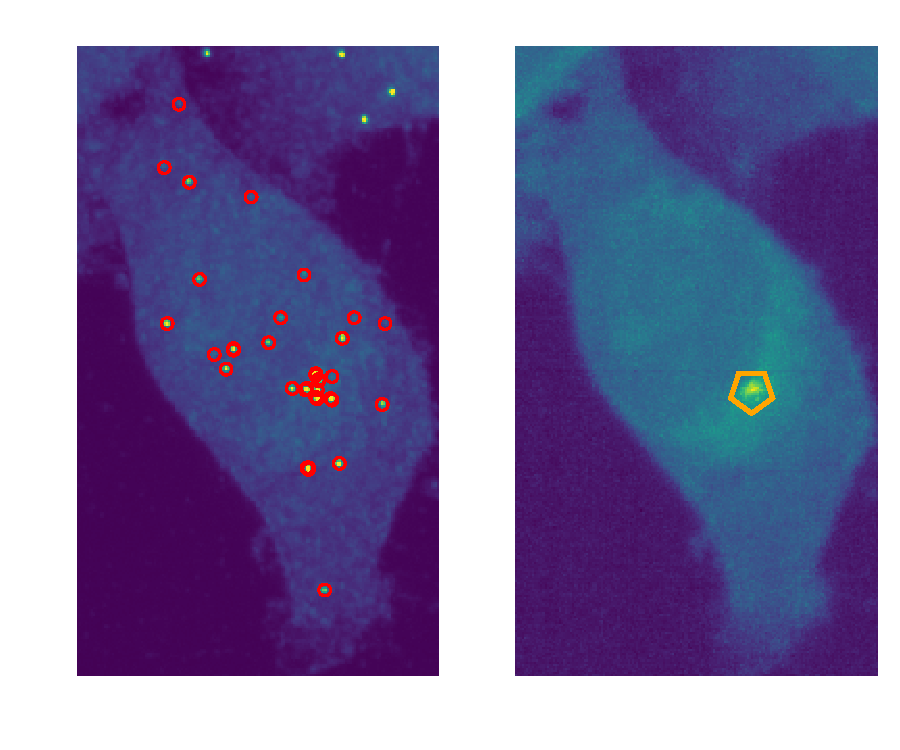
\includegraphics[width=\textwidth]{figures/chapter5/centrosomes}
    \caption{Contrasted image with detected RNAs on a smFISH channel (\textit{left}) and detected centrosome on a GFP channel (\textit{right}).
	Targeted transcript is BICD2.
	Plot build with \emph{bigfish}}
    \label{fig:centrosomes}
\end{figure}

\subsection{Materials and methods}
\label{subsec:materials_centrosomal}

\subsubsection{Experimental data}

\begin{figure}[]
    \centering
    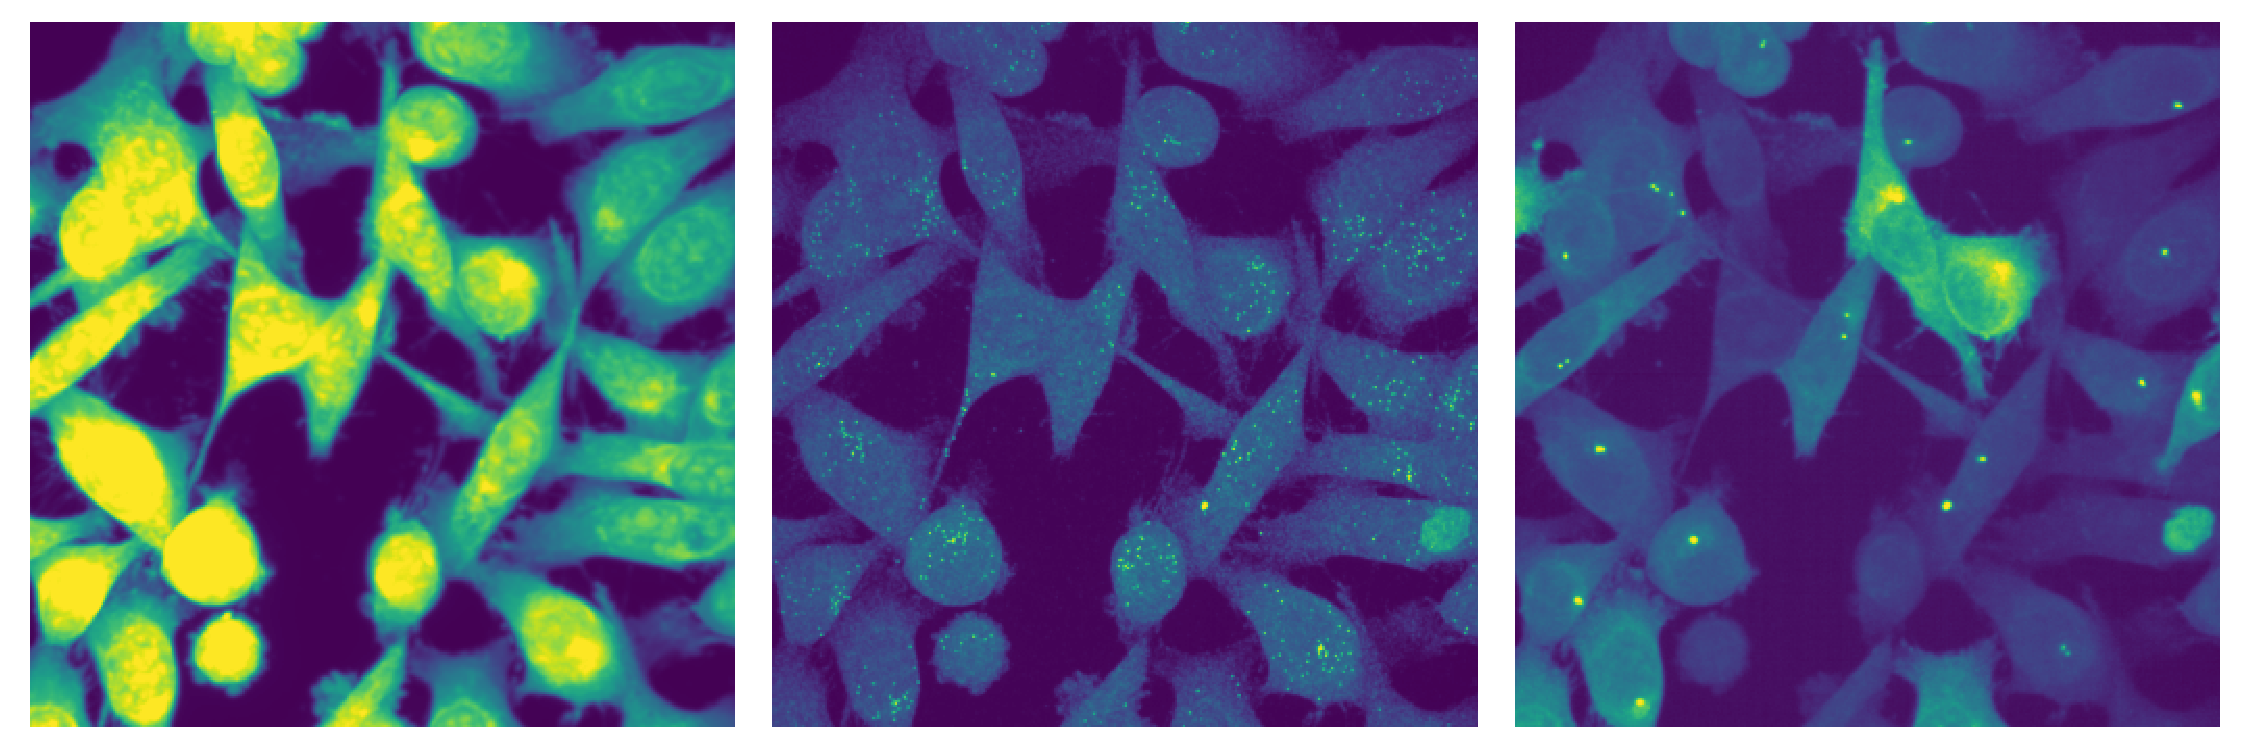
\includegraphics[width=\textwidth]{figures/chapter5/FoV_BICD2}
    \caption{Contrasted image with CellMask\textsuperscript{\texttrademark} (\textit{left}), smFISH (\textit{center}) and GFP (\textit{right}) channels.
	Targeted transcript is BICD2.
	Images are projected in 2D.
	Plot build with \emph{bigfish}}
    \label{fig:fov_adham}
\end{figure}

\subsubsection{Centrosome detection}

\subsubsection{Cell and nucleus segmentation}

\subsection{Results}
\label{subsec:results_centrosomal}

\subsubsection{Centrosomal mRNAs}

\begin{figure}[]
    \centering
    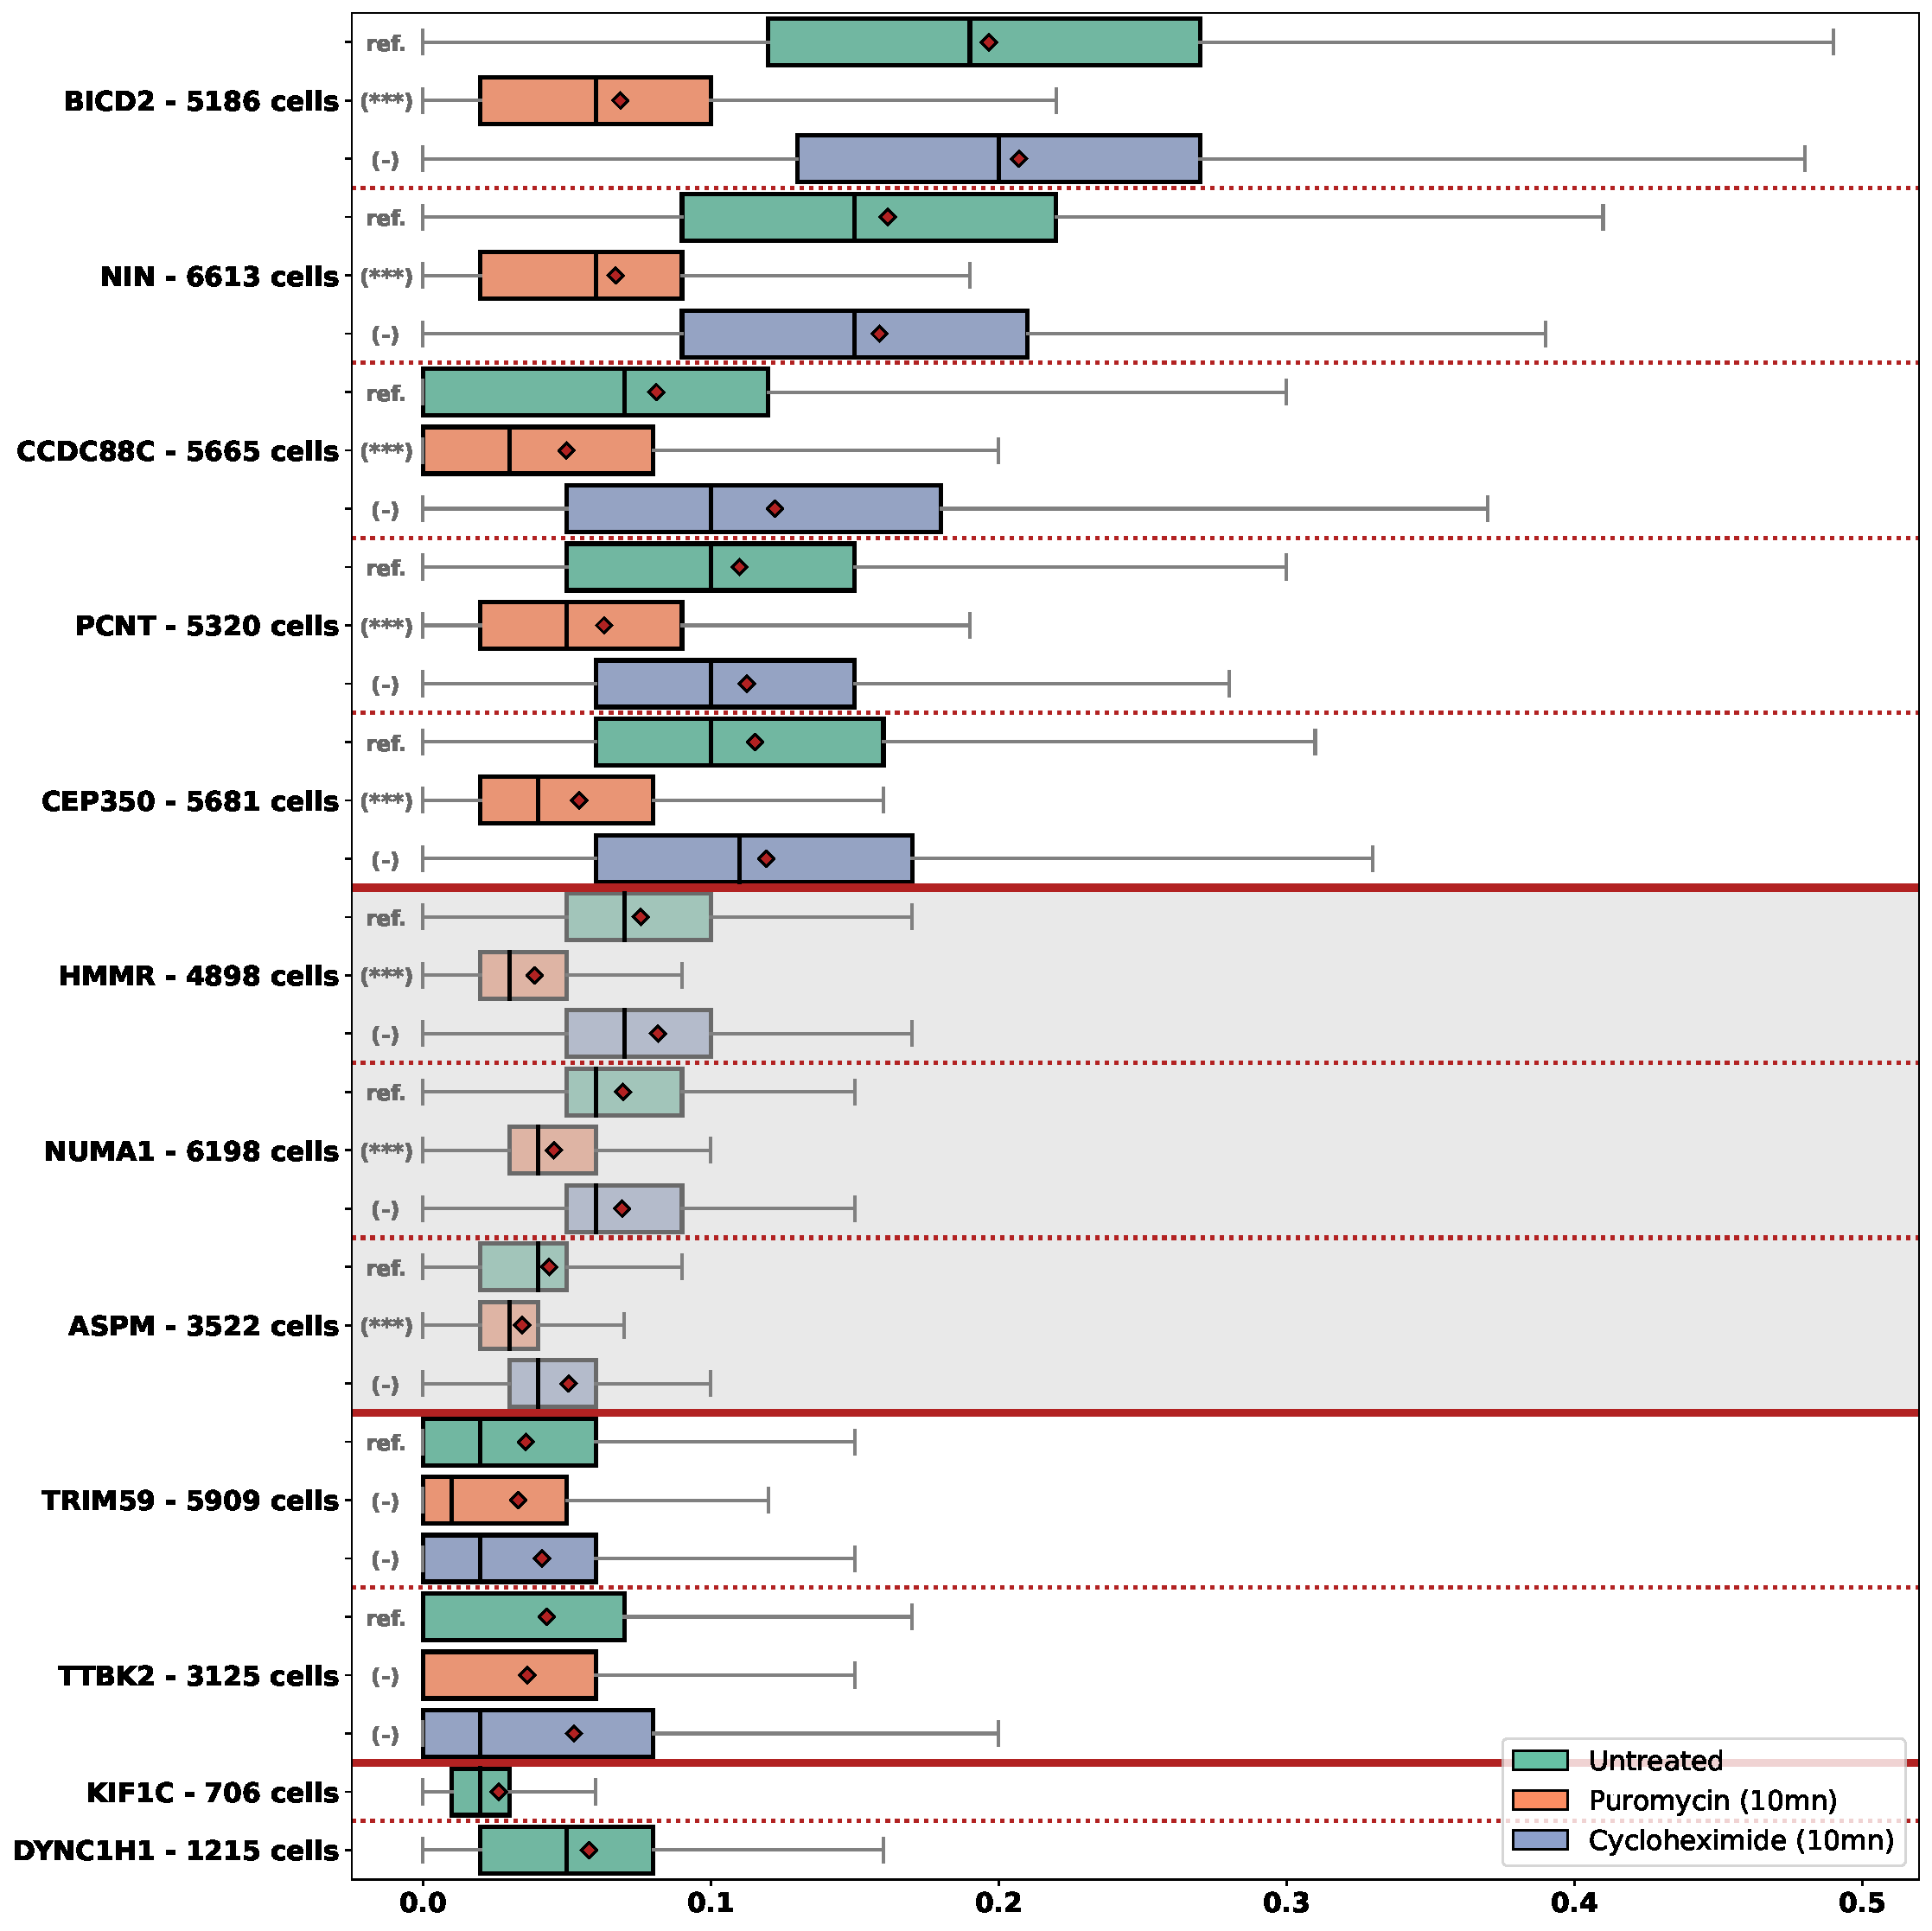
\includegraphics[width=\textwidth]{figures/chapter5/plot_rna_centrosome}
    \caption{Box plot with the proportion of centrosomal mRNAs in cells, for different genes and treatments.
	The \textit{whiskers} equal 1.5 the interquartile range.
	HMMR (in \textit{gray}) is an endogenous centrosomal mRNAs, the rest are BAC-transcribed mRNAs.
	A one-sided Welch’s t test is used to evaluate significance}
    \label{fig:plot_rna_centrosome}
\end{figure}

% Box plots depicting the proportion of centrosomal mRNAs in cells (interphase and mitotic),
% for the indicated mRNAs and cell treatments. Values were computed for each cell and the
% number of cells analyzed is indicated. The distribution of the values is depicted in the boxed plot.
% The colored area corresponds to the second and third quartiles, the mean to the black vertical bar,
% and the median to the red diamond. The whiskers equal 1.5 the interquartile range.
% The right graph represents endogenous centrosomal mRNAs, while the left one represents
% BAC-transcribed mRNAs. Significance was evaluated with a one-sided Welch’s t test.
% ***: null hypothesis rejected with a 0.1% significance level, and -: null hypothesis not rejected.

\subsubsection{Influence of mitosis}

%%%%%%%%%%%%%%%%%%%%%%%%%%%%%%%%%%%%%%%%%%%%%%%%%%%%%%%%%%%%%%%%%%%%%%%%%%%%%%%%%%%%%%%%%%%%%%%%%%%%%%%%%%%%%%%%%%%%%%%%%%%%%%%%%%%%%%%%%%%%%%%%%%%%%%%%%%%%
%%%%%%%%%%%%%%%%%%%%%%%%%%%%%%%%%%%%%%%%%%%%%%%%%%%%%%%%%%%%%%%%%%%%%%%%%%%%%%%%%%%%%%%%%%%%%%%%%%%%%%%%%%%%%%%%%%%%%%%%%%%%%%%%%%%%%%%%%%%%%%%%%%%%%%%%%%%%
%%%%%%%%%%%%%%%%%%%%%%%%%%%%%%%%%%%%%%%%%%%%%%%%%%%%%%%%%%%%%%%%%%%%%%%%%%%%%%%%%%%%%%%%%%%%%%%%%%%%%%%%%%%%%%%%%%%%%%%%%%%%%%%%%%%%%%%%%%%%%%%%%%%%%%%%%%%%

\section{Protrusion pattern}
\label{sec:protrusion}

\begin{center}
	\textit{(To be completed)}
\end{center}

% paper racha (transript encoding motors)

% Surprisingly, the proteins encoded by some of these localized mRNAs did not appear strongly enriched at the site of mRNA accumula- tion.
% GFP-KIF4A was mostly nuclear with only a faint staining at the cell periphery, while GFP-tagged KIF5B, DYNLL2, and DYNC1H1 proteins
% localized throughout the cytoplasm without a specific enrichment in protrusions or foci (Figure 1). Co-locali- zation was only observed for KIF1C-GFP, where both the mRNA
% and the GFP-tagged protein accumulated in cytoplasmic protru- sions. This suggested that the KIF1C-GFP mRNAs were trans- lated locally.

% To confirm the BAC results, endogenous mRNAs were analyzed using smiFISH, an inexpensive variant of smFISH (Tsa- nov et al., 2016).
% KIF1C mRNAs accumulated in cytoplasmic pro- trusions in all the examined cell lines, including human HeLa cells as well as mouse
% 3T3 fibroblasts and C2C12 myoblasts (Fig- ure S2A). Furthermore, in differentiated SH-SY5Y neuronal cells, KIF1C mRNA localized
% in dendritic-like outgrowths, away from the cell body, while a control CRM1 mRNA remained in the soma (Figure S2B)

% To provide a quantitative view of mRNA localization, we developed tools to identify the cytoplasmic protrusions, and we
% measured both the fraction of cytoplasmic mRNAs located in this compartment and their enrichment as compared with a uniform
% distribution of molecules (see STAR Methods). This re- vealed a high heterogeneity of mRNA localization in protrusions,
% with values varying from 0\% to 60\% of the molecules depending on the cell (Figure S3A).
% On average, the enrichment in protru- sions of KIF1C, KIF4A, DYNLL2, and MYH3 mRNAs was several folds higher than for
% control motor mRNAs annotated as random (KIF20B and MYO18A; Figure S3A). It was, however, lower than for RAB13 mRNA
% that we used as a positive control (Mili et al., 2008). Next, we determined whether KIF1C, KIF5B, MYH3, and KIF4A mRNAs accumulated in the same protrusions.
% Two-color smFISH against the endogenous KIF1C mRNAs and the BAC- tagged mRNAs revealed that this was indeed the case (Fig- ure S3B).

\subsection{Introduction}
\label{subsec:introduction_protrusion}

\subsection{Materials and methods}
\label{subsec:materials_protrusion}

\subsection{Results}
\label{subsec:results_protrusion}

\begin{figure}[h]
    \centering
    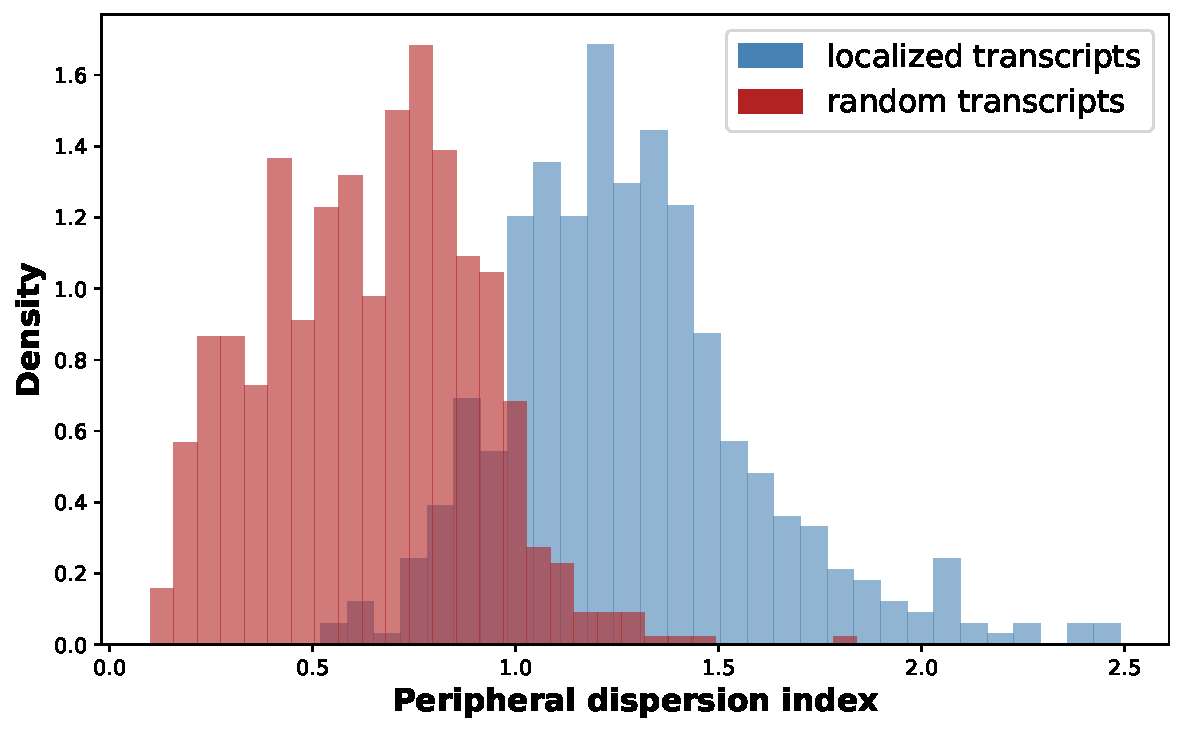
\includegraphics[width=\textwidth]{figures/chapter5/helacentrin_distribution_pdi}
    \caption{Blablabla}
    \label{fig:xavier_pdi}
\end{figure}

\section{Exploring large scale dataset}
\label{sec:exploration}

\begin{center}
	\textit{(To be completed)}
\end{center}

%~\cite{lecuyer_global_2007}

%To address this point, we developed and employed a high-resolution fluorescent
%in situ hybridization procedure to comprehensively evaluate mRNA localization
%dynamics during early Drosophila embryogenesis. Surprisingly, of the 3370 genes
%analyzed, 71\% of those expressed encode subcellularly localized mRNAs.
%Dozens of new and striking localization patterns were observed, implying an
%equivalent variety of localization mechanisms. Tight correlations between mRNA
%distribution and subsequent protein localization and function, indicate major
%roles for mRNA localization in nucleating localized cellular machineries.

%Computational Analysis The annotation data was converted into a binary matrix,
%containing genes on one axis and localization terms on the other, where the presence
%of a localization feature for a given gene was indicated numerically as ‘‘1,’’
%while lack of a feature was annotated as ‘‘0.’’ This matrix was then used for GO
%term enrichment analysis. Functional GO annotations for all genes were downloaded
%from Flybase (http://flybase.bio. indiana.edu/genes/lk/function/). Annotations
%were up-propagated using the GO hierarchy (Ashburner et al., 2000), and calculations
%were restricted to genes that were both GO annotated and analyzed in this study
%(1651 genes). The hypergeometric distribution was used to calculate probabilities
%of overlap between each localization category against all GO categories containing
%three or more genes. The Benjamini-Hochberg procedure (Benjamini and Hochberg, 1995)
%was used to control for multiple testing by computing a P-value threshold
%corresponding to a false discovery rate (FDR) of 0.25. Transcript subgroups
%were also analyzed independently for GO term enrichments using EASE (Hosack et al., 2003).
%EASE scores of less that 0.05 were considered significant, as reported previously (Tadros et al., 2007a).

\section{Conclusion}
\label{sec:conclusion_chapter5}

\begin{center}
	\textit{(To be completed)}
\end{center}

% racha paper

% In conclusion, this quantitative analysis corroborated the manual annotations and revealed a high degree of heterogeneity of RNA localization across different cells.
% This heterogeneity is a general phenomenon since it is seen with nearly all the genes analyzed here.

% racha paper (discussion)

% In this study, we performed a dual RNA-protein localization screen and analyzed more than 500 genes.
% We found 32 localized mRNAs, with 15 accumulating in P-bodies and the others being locally translated
% (Table 1). We also discovered a number of unexpected features, and in particular that: (1) co-translational
% mRNA targeting is frequent and occurs at unexpected locations; and (2) mRNAs can be translated in specialized
% translation fac- tories, defined as a polysome aggregates. These factories can perform specific tasks on nascent proteins.
% Localization of mRNA Shows a High Degree of Heterogeneity in Cell Lines
% Co-translational RNA Targeting Occurs in Multiple Subcellular Locations
% A Specific Translational Program Occurs at Mitotic Centrosomes
% P-Bodies and Translation Factories

% adham paper

% xavier paper

